\documentclass[usenames,dvipsnames,11pt,aspectratio=169]{beamer}
\usepackage{ifthen}
\usepackage{xcolor}
\usepackage{pgfplots}
\usepackage{amsmath}
\usepackage{centernot}
\usepackage{pifont}
\usepackage{tabularx}
\usepackage{makecell}
\usepackage{cuted}
\usepackage{subcaption}
\usepackage{booktabs}
\usepackage{array}
\usepackage{textcomp}
\usepackage{setspace}
\usepackage{xspace}
\usepackage{tikz}
\usepackage{pdfcomment}
%\newcommand{\pdfnote}[1]{\marginnote{\pdfcomment[icon=note]{#1}}}
\newcommand{\pdfnote}[1]{}

\usepackage{pgfpages}
%\setbeameroption{show notes on second screen}


\input ../beamer-style
\input ../std-macros
\input ../macros

\AtBeginSection[]
{
    \begin{frame}
        \frametitle{Table of Contents}
        \tableofcontents[currentsection]
    \end{frame}
}
\parskip=10pt

\title[CSCI-GA.2590]{Representation Learning}
\author[He He]{He He
}
\institute[NYU]{New York University}
\date{November 17, 2021}

\begin{document}
\begin{frame}
\titlepage
\end{frame}

\section{Transformers}

\begin{frame}
    {Recap: BiLSTM}
    \begin{figure}
        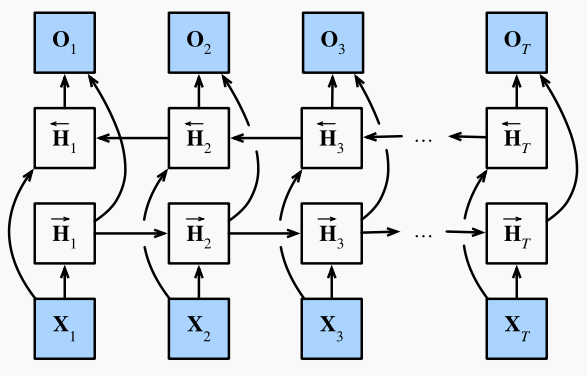
\includegraphics[height=4cm]{figures/bilstm}
    \end{figure}
    \begin{itemize}
        \item Classification: $p(y\mid x) = \text{softmax}(\text{linear}(\text{pooling}(o_1,\ldots,o_T)))$
        \item Sequence labeling: $p(y_t\mid x) = \text{softmax}(\text{linear}(o_t))$
        \item Sequence generation: decoder + attention
    \end{itemize}
\end{frame}

\begin{frame}
    {Tasks with two inputs}
    \beamerblue{Natural language inference}\\
    \begin{itemize}
        \item[] Premise: 8 million in relief in the form of emergency housing.
        \item[] Hypothesis: The 8 million dollars for emergency housing was still not enough to solve the problem. 
        \item[] Label: neutral
    \end{itemize}

    \beamerblue{Reading comprehension}\\
    \begin{itemize}
        \item[] 
        {\small
        Super Bowl 50 was an American football game to determine the champion of the National Football League (NFL) for the 2015 season. The American Football Conference (AFC) champion \emph{Denver Broncos} defeated the National Football Conference (NFC) champion Carolina Panthers 24--10 to earn their third Super Bowl title. The game was played on February 7, 2016, at Levi's Stadium in the San Francisco Bay Area at Santa Clara, California.}
\item[] Question: Which team won Super Bowl 50?
\item[] Answer: Denver Broncos 
    \end{itemize}
\end{frame}

\begin{frame}
    {Encode two inputs}
    \beamerblue{Goal}: $\sX \times \sX \rightarrow \sY$

    Simple combination:\\
    \begin{itemize}
        \item Encode $x_1$ and $x_2$ in $\BR^d$ separately
        \item Aggregate the two embeddings, e.g. $\text{MLP}(\text{pooling}(\text{enc}(x_1), \text{enc}(x_2)))$
        \item Pooling: concatenation, elementwise max, elementwise product etc.
        \item \green{Modular}, but \red{less expressive}
    \end{itemize}

    Finer-grained interaction between the two inputs:\\
    \begin{itemize}
        \item Can we use something similar to the attention mechanism in seq2seq?
    \end{itemize}
            \vspace{7em}
\end{frame}

\begin{frame}
    {BiDAF}
    Bi-Directional Attention Flow for Machine Comprehension [Seo+ 2017]\\
    \beamerblue{Key idea}: representation of $x_1$ depends on $x_2$ and vice versa
    \vspace{-1em}
    \begin{figure}
        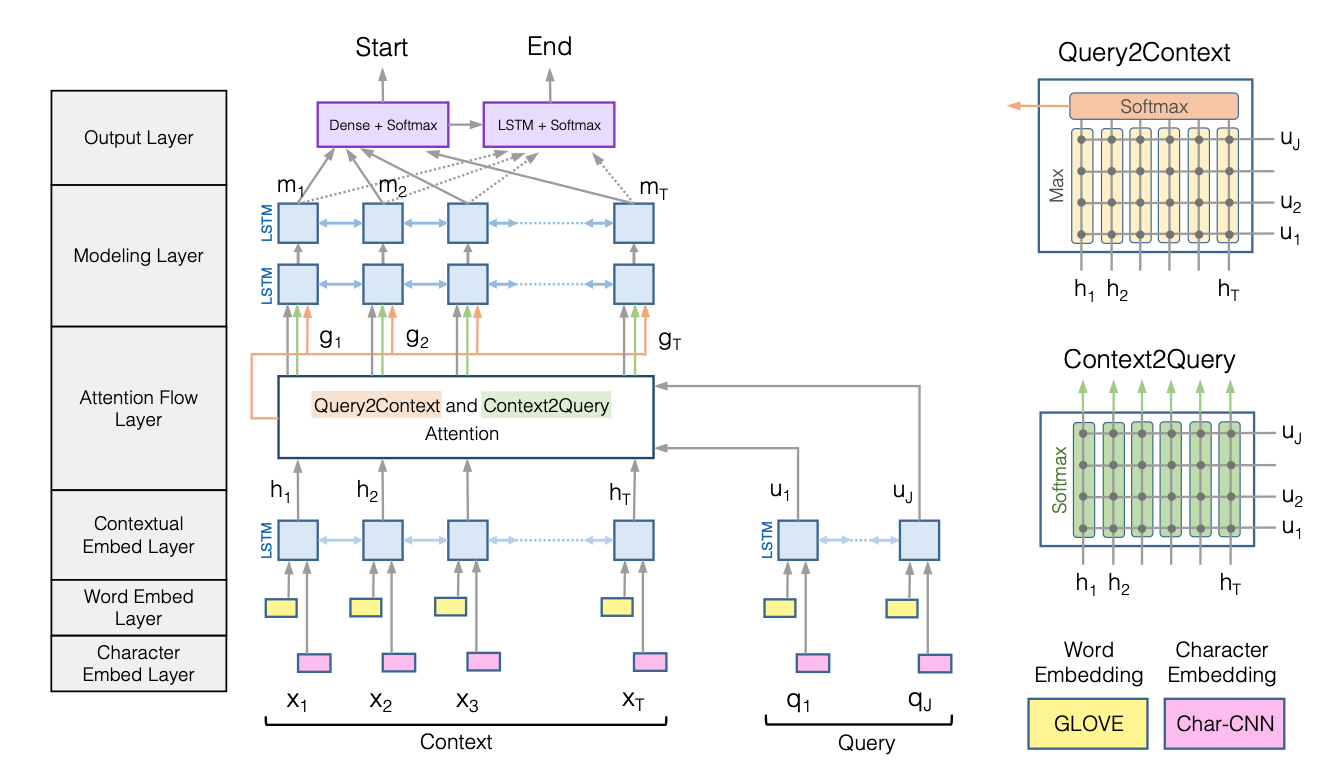
\includegraphics[height=7cm]{figures/bidaf}
    \end{figure}
\end{frame}

\begin{frame}
    {Improve the efficiency of RNNs}
    \beamerblue{Word embedding}: represents the meaning of a word 

    \beamerblue{Recurrent neural networks}: captures dependence among words in a sentence 

    \beamerblue{Attention mechanism}: better modeling of long-range dependence 

    Multi-layer biLSTM with various attentions was the go-to architecture for most NLP tasks.

    {But}, RNNs are \red{sequential} and difficult to scale up\\
    \begin{itemize}
        \item[] We want deeper models trained with larger data.
    \end{itemize}

    Can we handle dependencies in a more \green{efficient} way?
\end{frame}

\begin{frame}
    {Attention is all you need?}
    Key idea: get rid of recurrence and only rely on attention
    \begin{figure}
        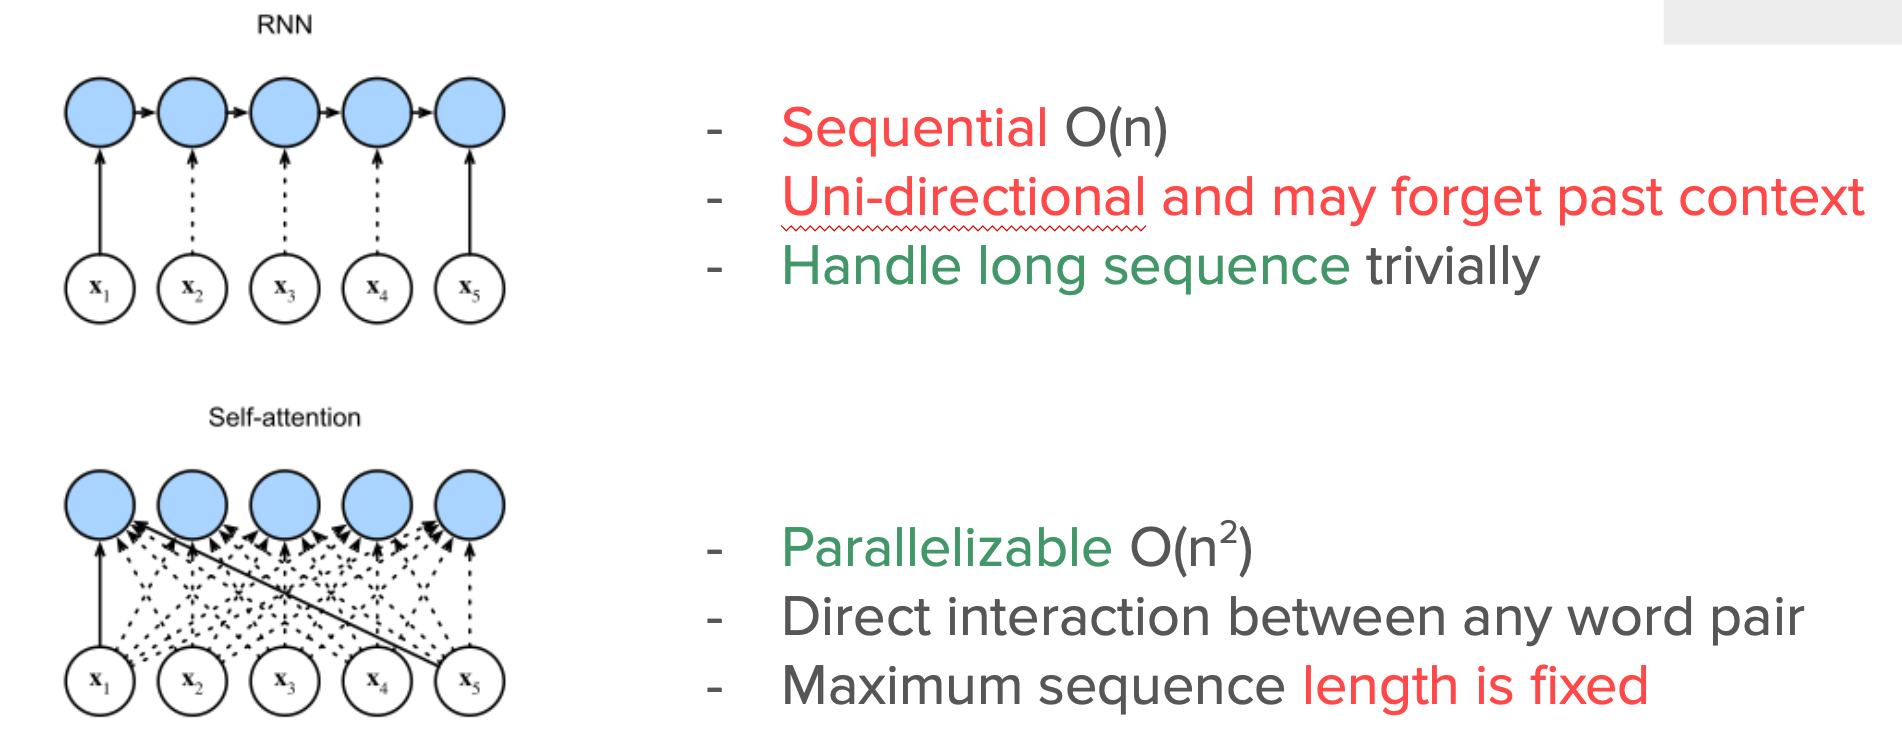
\includegraphics[height=5cm]{figures/rnn-vs-attn}
    \end{figure}
\end{frame}

\begin{frame}
    {Transformer overview}
    Attention is all you need. [Vaswani+ 2017]

    Replaces recurrence with self-attention:\\
    \begin{figure}
        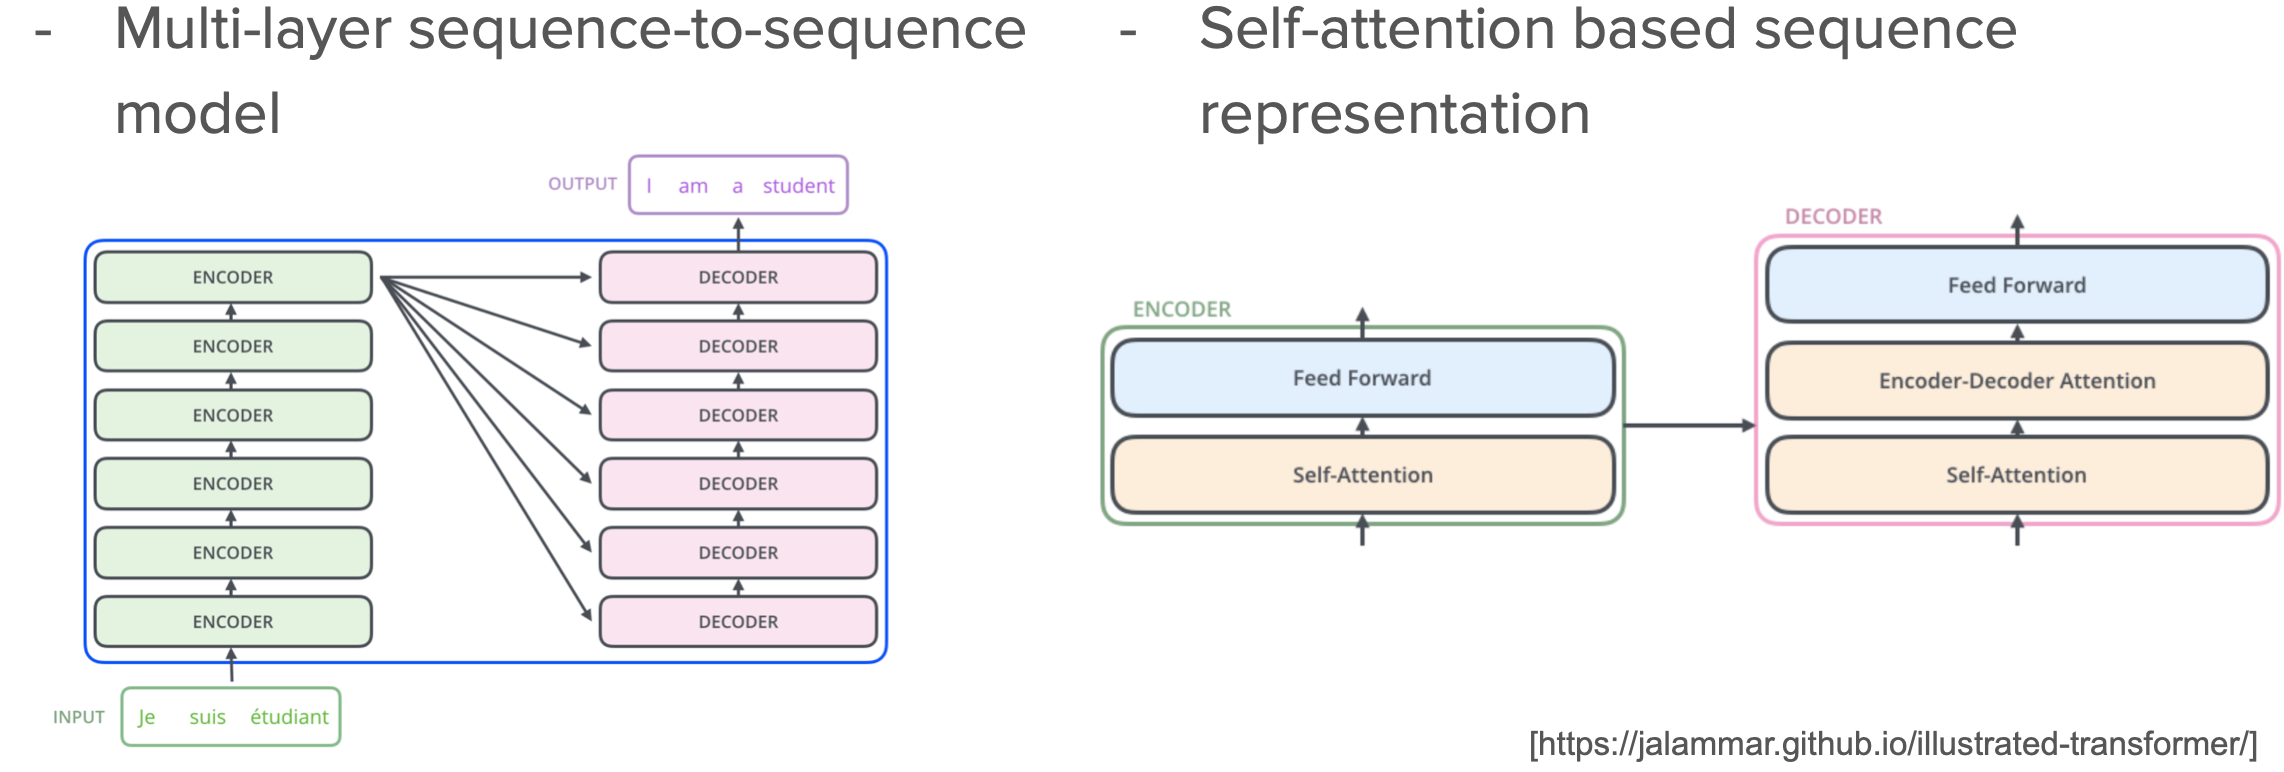
\includegraphics[width=\textwidth]{figures/transformer-high-level}
    \end{figure}
    %\begin{itemize}
    %    \item \beamerblue{Self-attention}: an attention memory of the input sequence for each token in the input sequence (parallelizable)
    %    \item \beamerblue{Position embedding}: models sequential information (doesn't lose word order)
    %\end{itemize}

    %Other key components:\\
    %\begin{itemize}
    %    \item Multi-head attention
    %    \item Residual connection and layer norm: improves optimization of deep models
    %\end{itemize}
\end{frame}

\begin{frame}
    {Transformer block}
    \begin{figure}
        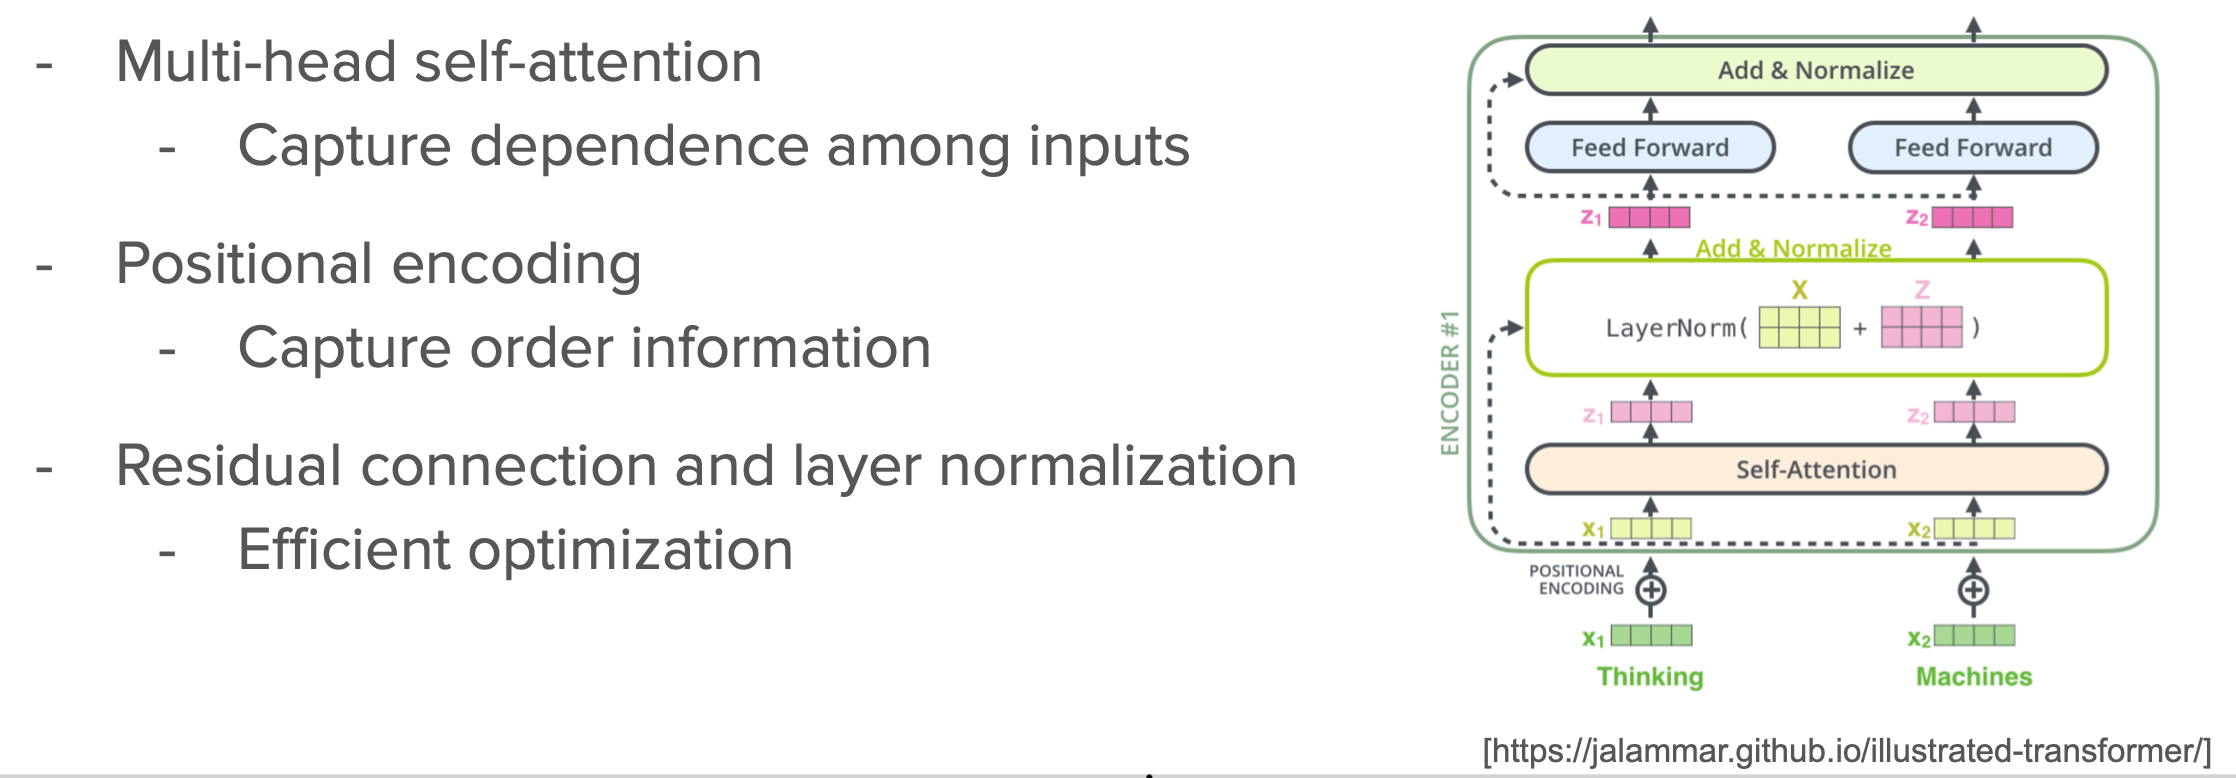
\includegraphics[width=\textwidth]{figures/transformer-block}
    \end{figure}
\end{frame}

\begin{frame}
    {Self-attention}
    \begin{figure}
        \begin{subfigure}{.5\textwidth}
        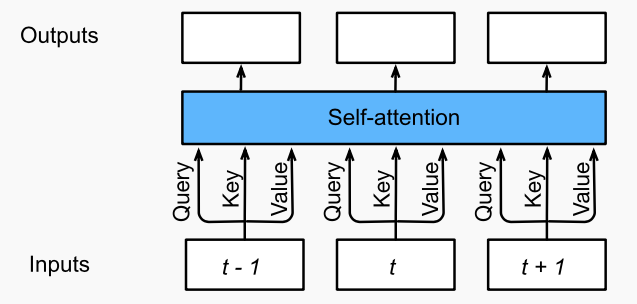
\includegraphics[height=3cm]{figures/self-attn}
        \end{subfigure}
        \begin{subfigure}{.4\textwidth}
        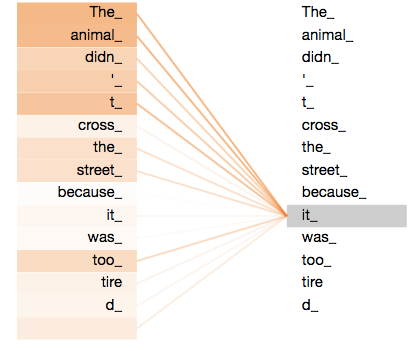
\includegraphics[height=3cm]{figures/self-attn-ex}
        \end{subfigure}
    \end{figure}
    \begin{itemize}
        \item Seq2seq attention: keys and values are the input words, and queries are the output (prefix).
        \item Self-attention: keys, values, and queries are all from the input words.
            \begin{itemize}
                \item Input: a sequence of words
                \item Output: (contextualized) embeddings for each word
            \end{itemize}
        \item Each word (as a query) interacts with all words (keys/values) in the input
        \item Computation of the attention output for each word can be parallelized
    \end{itemize}
\end{frame}

\begin{frame}
    {Matrix representation}
    \begin{figure}
        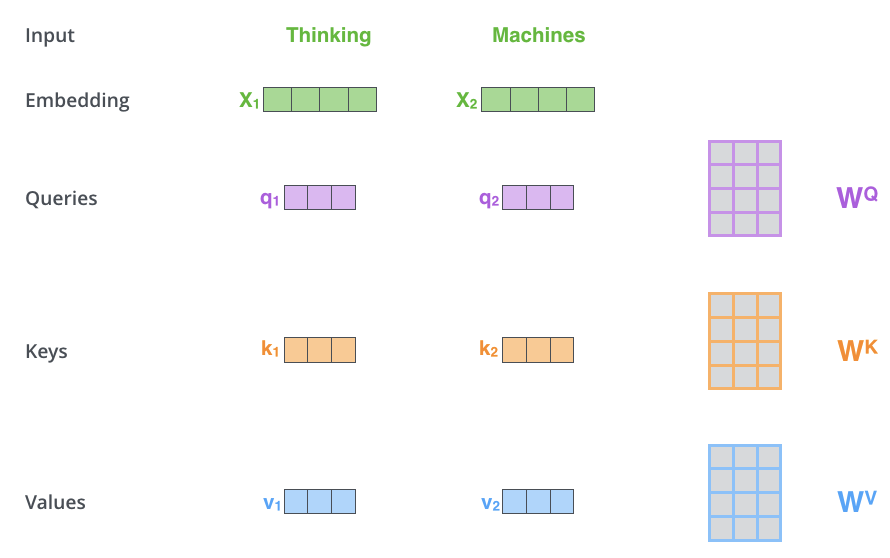
\includegraphics[height=7cm]{figures/self-attn-matrix.png}
        \caption{From ``The Illustrated Transformer''}
    \end{figure}
\end{frame}

\begin{frame}
    {Scaled dot-product attention}
    \textbf{Scaled dot-product attention}
    $$
     \alpha(q, k) = q \cdot k / \sqrt{d} 
    $$
    \vspace{-3em}
    \begin{itemize}
        \item $\sqrt{d}$: dimension of the key vector
        \item Avoids large attention weights that push the softmax function into regions of small gradients
    \end{itemize}
    \vspace{-1em}
    \begin{figure}
        \begin{subfigure}{.4\textwidth}
        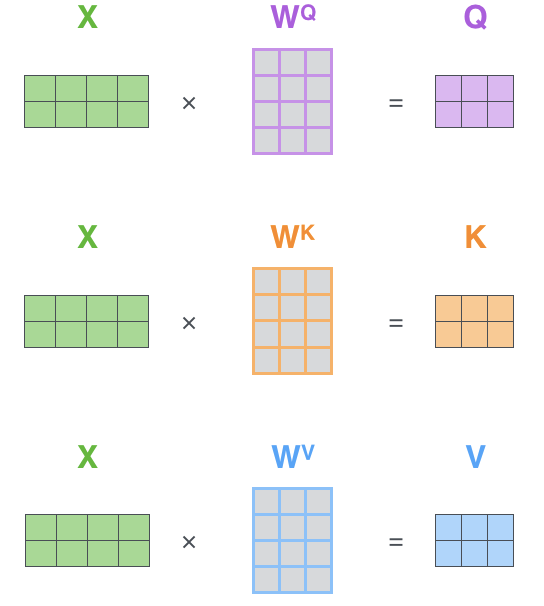
\includegraphics[height=4cm]{figures/scaled-attn}
        \end{subfigure}
        \begin{subfigure}{.5\textwidth}
        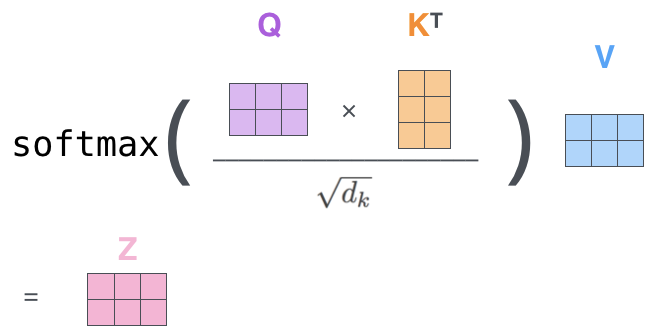
\includegraphics[height=3cm]{figures/scaled-attn-2}
        \end{subfigure}
    \end{figure}
\end{frame}

\begin{frame}
    {Multi-head attention: motivation}
    \begin{center}
        \textit{Time flies like an arrow}
    \end{center}
    \begin{itemize}
        \item Each word attends to all other words in the sentence
        \item Which words should ``like'' attend to?
            \begin{itemize}
                \item Syntax: ``flies'', ``arrow'' (a preposition)
                \item Semantics: ``time'', ``arrow'' (a metaphor)
            \end{itemize}
        \item We want to represent different roles of a word in the sentence: need more than a single embedding
        \item Instantiation: multiple self-attention modules
    \end{itemize}
\end{frame}

\begin{frame}
    {Multi-head attention}
    \begin{figure}
        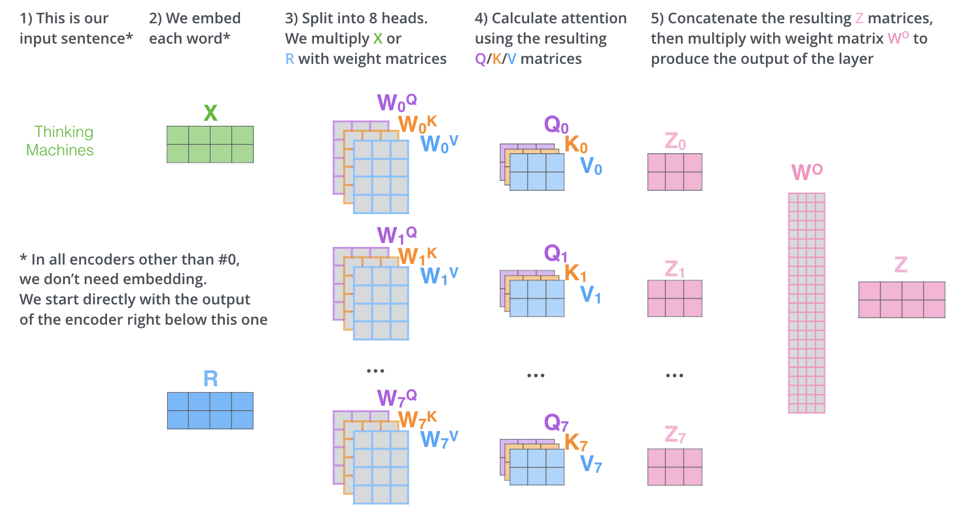
\includegraphics[width=.9\textwidth]{figures/multi-head}
    \end{figure}
\end{frame}

\begin{frame}
    {Time complexity}
    \begin{figure}
        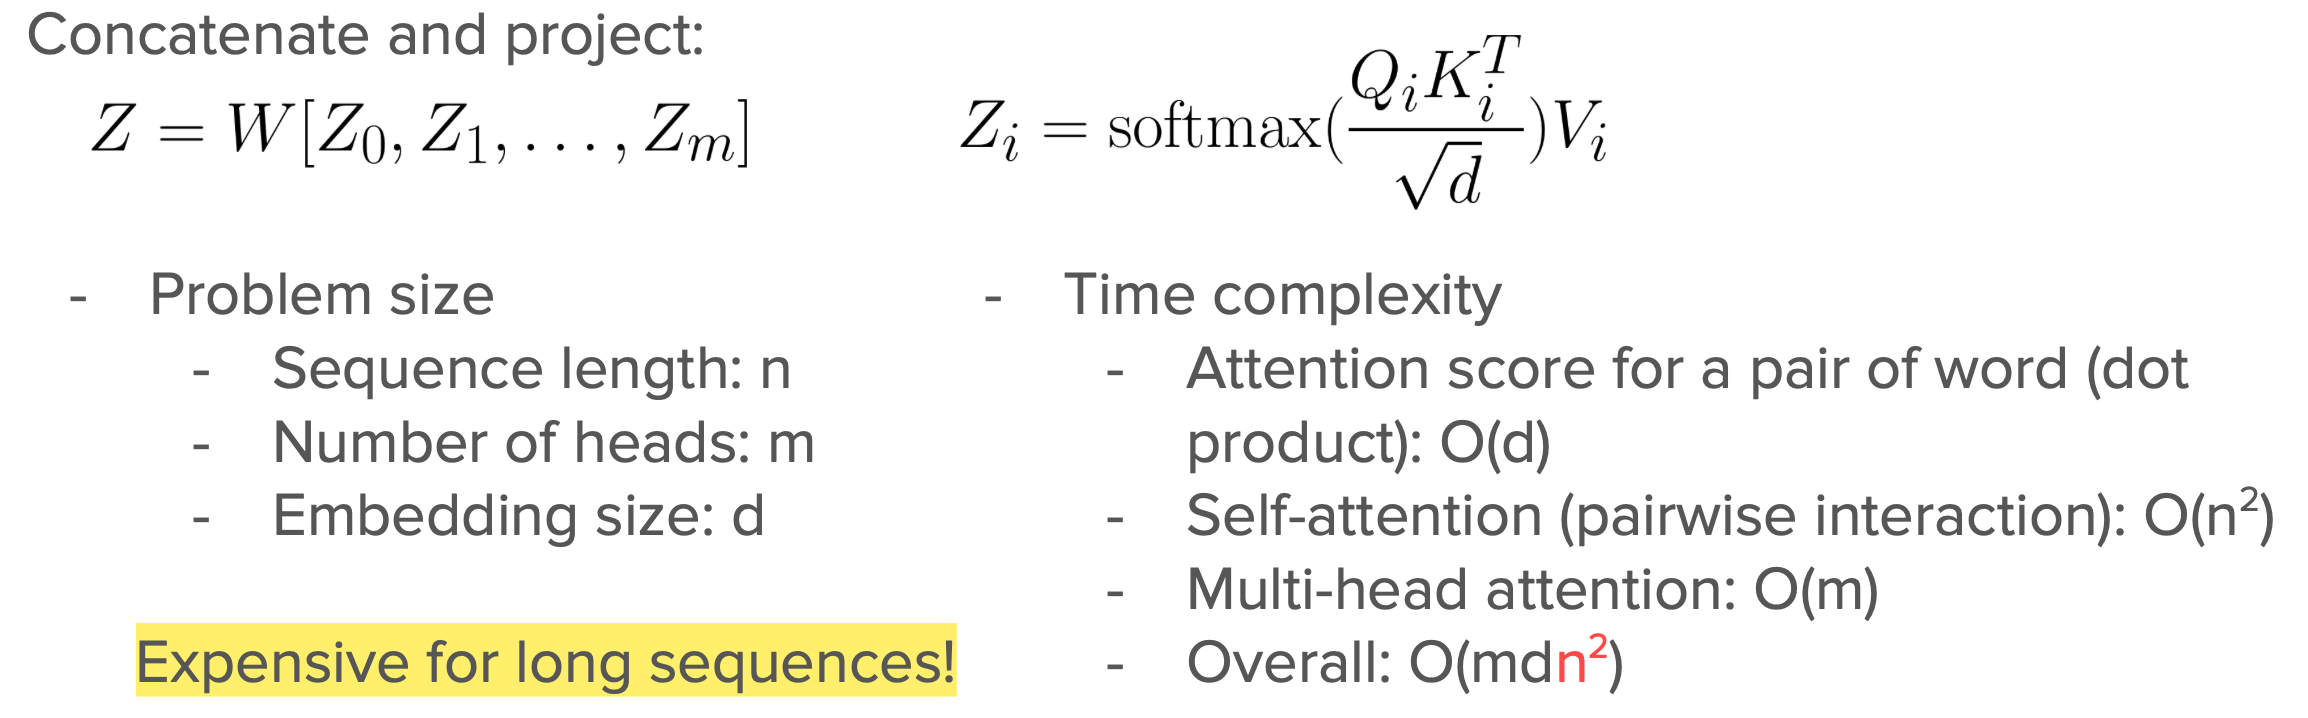
\includegraphics[width=\textwidth]{figures/multihead-time}
    \end{figure}
\end{frame}

\begin{frame}
    {Efficient self-attention}
    \begin{figure}
        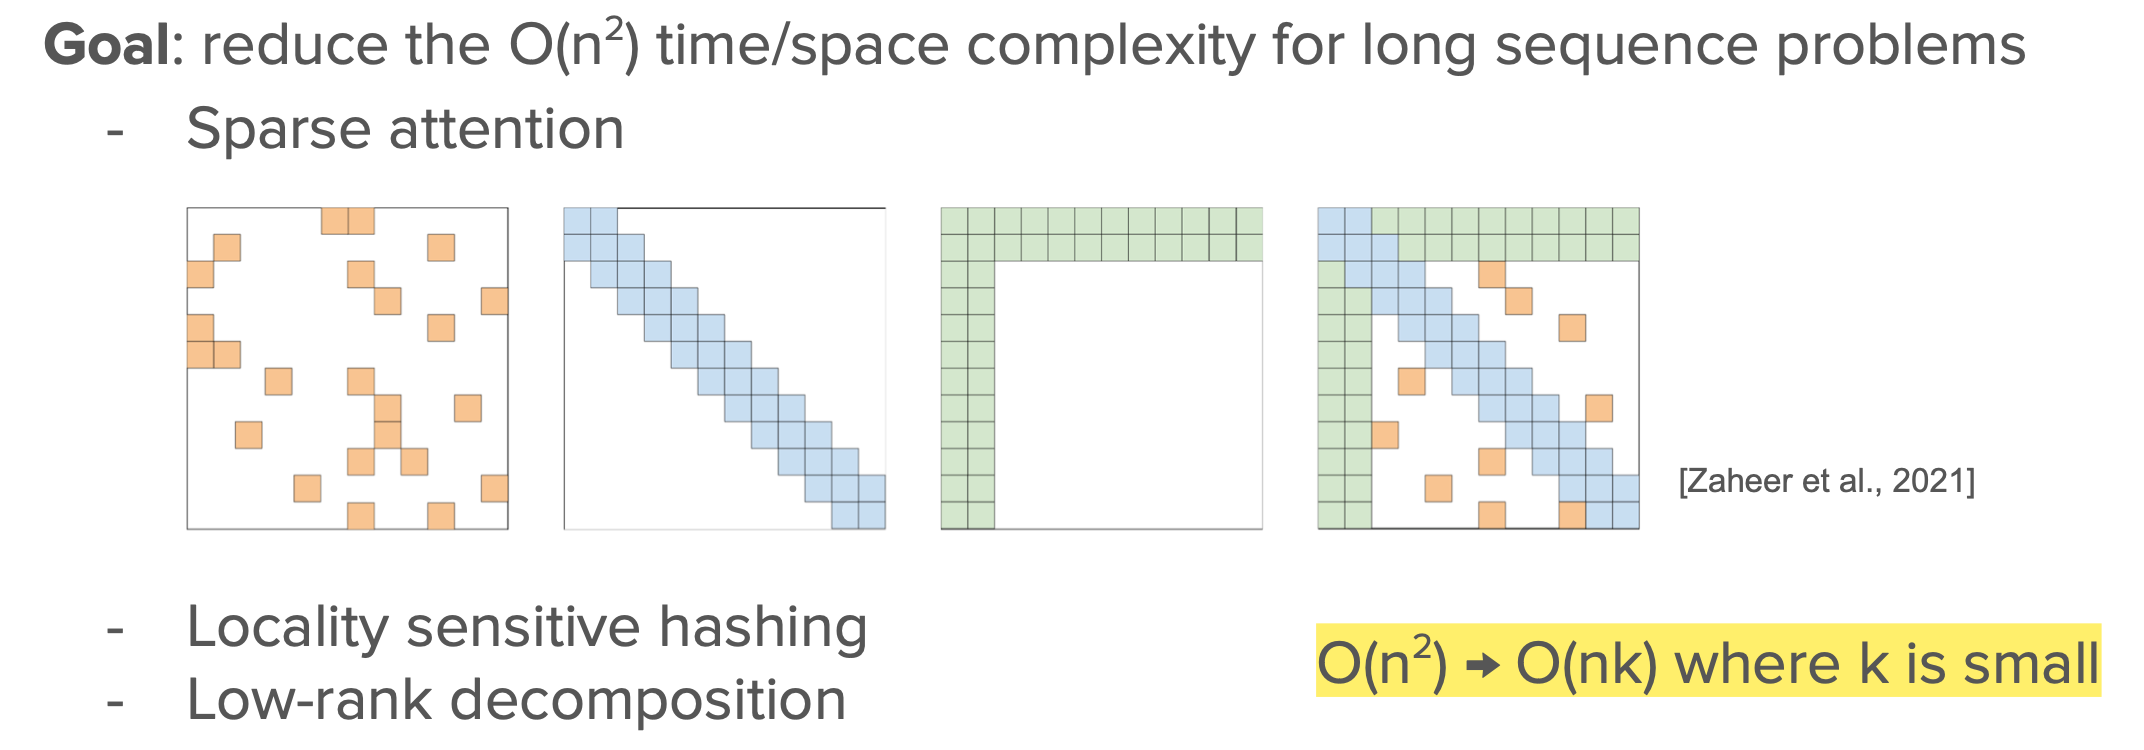
\includegraphics[width=\textwidth]{figures/efficient}
    \end{figure}
\end{frame}

\begin{frame}
    {Position embedding}
    Motivation: model word order in the input sequence

    Solution: add a position embedding to each word
    \begin{figure}
        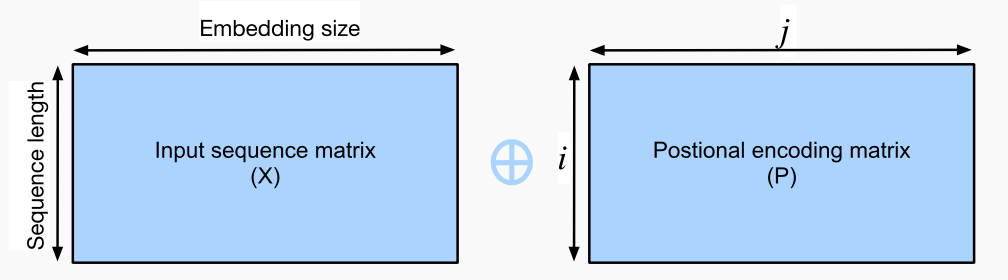
\includegraphics[height=3cm]{figures/position-embedding}
    \end{figure}

    Position embedding:\\
    \begin{itemize}
        \item Encode absolute and relative positions of a word
        \item (Same dimension as word embeddings)
        \item Learned or deterministic 
    \end{itemize}
\end{frame}

%\begin{frame}
%    {Sinusoidal position embedding}
%    \begin{itemize}
%        \item Same dimension as word embeddings
%        \item Two components ($2i, 2i+1$) represent a rotation vector: $\sin(\omega_{2i}t), \cos(\omega_{2i}t)$ ($t$ is the position)
%        \item Multiple rotation vectors with different angular velocities: $\omega_{2i}$
%        \item Analogous to binary encoding
%    \end{itemize}
%    \begin{figure}
%        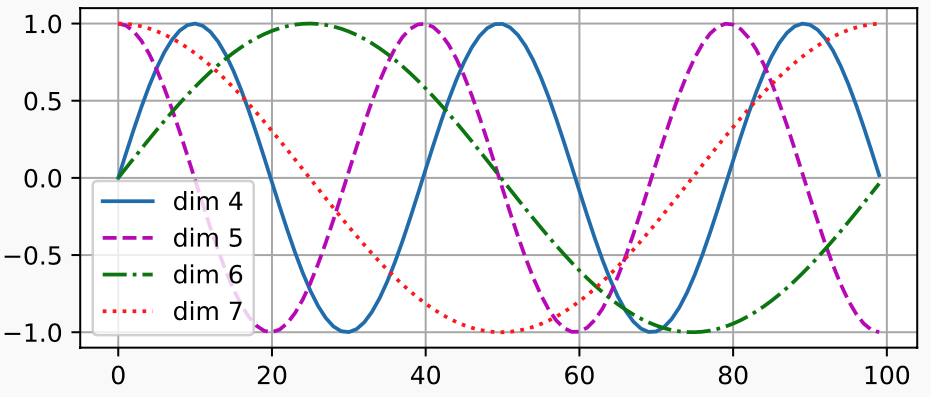
\includegraphics[height=3cm]{figures/sinusoidal}
%    \end{figure}
%\end{frame}

\begin{frame}
    {Sinusoidal position embedding}
    \begin{figure}
        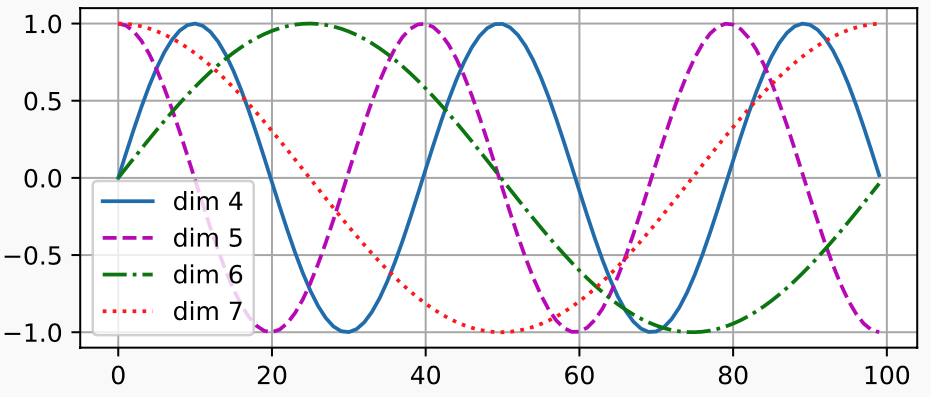
\includegraphics[width=\textwidth]{figures/sinusoidal}
    \end{figure}
\end{frame}

\begin{frame}
    {How important is word ordering?}
    \begin{figure}
        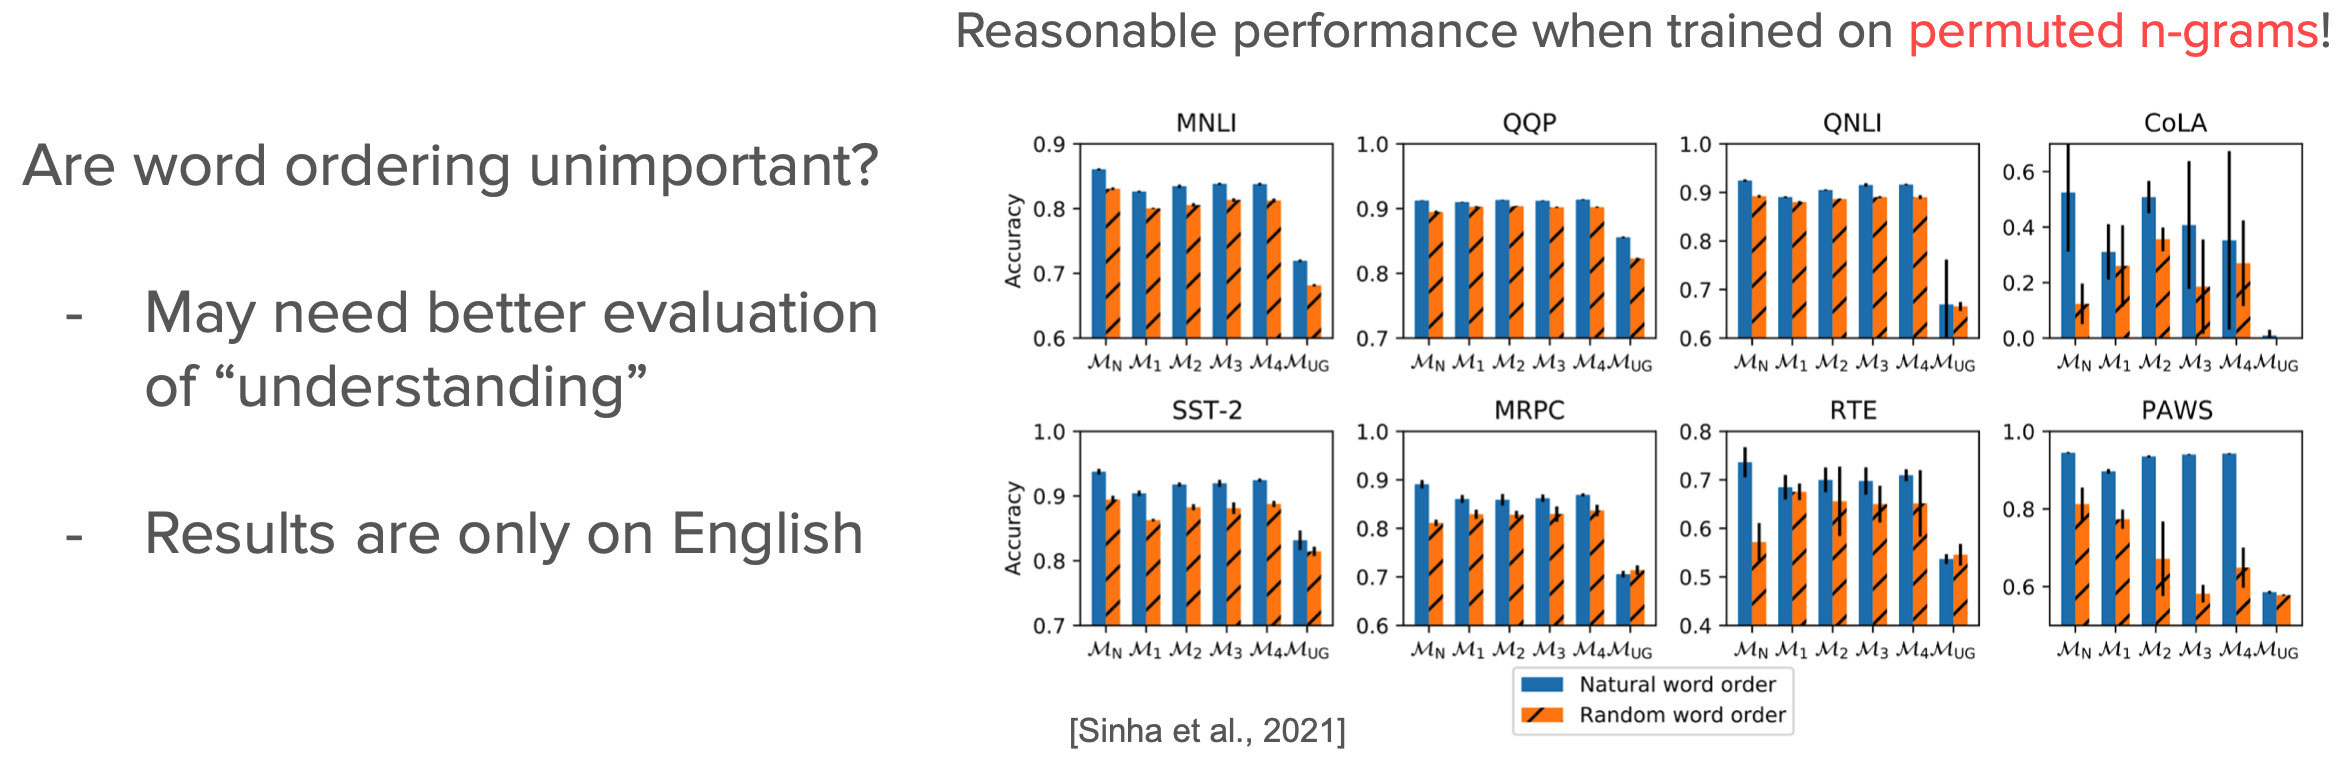
\includegraphics[width=\textwidth]{figures/permute}
    \end{figure}
\end{frame}

\begin{frame}
    {Residual connection and layer normalization}
    \begin{figure}
        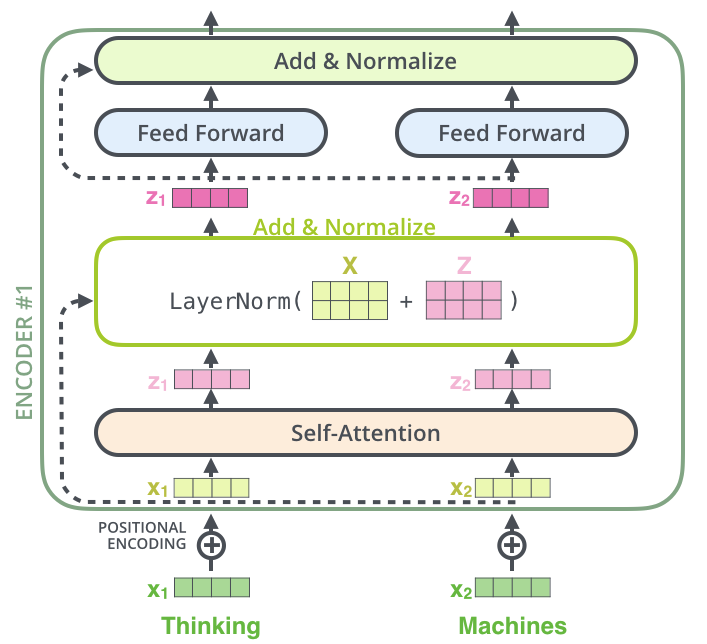
\includegraphics[height=5cm]{figures/add-norm}
    \end{figure}
    \vspace{-2em}
    \begin{itemize}
        \item Residual connection: add input to the output of each layer 
        \item Layer normalization: normalize (zero mean, unit variance) over all features for each sample in the batch
        \item Position-wise feed-forward networks: same mapping for all positions
    \end{itemize}
\end{frame}

\begin{frame}
    {Connect the decoder}
    \begin{figure}
        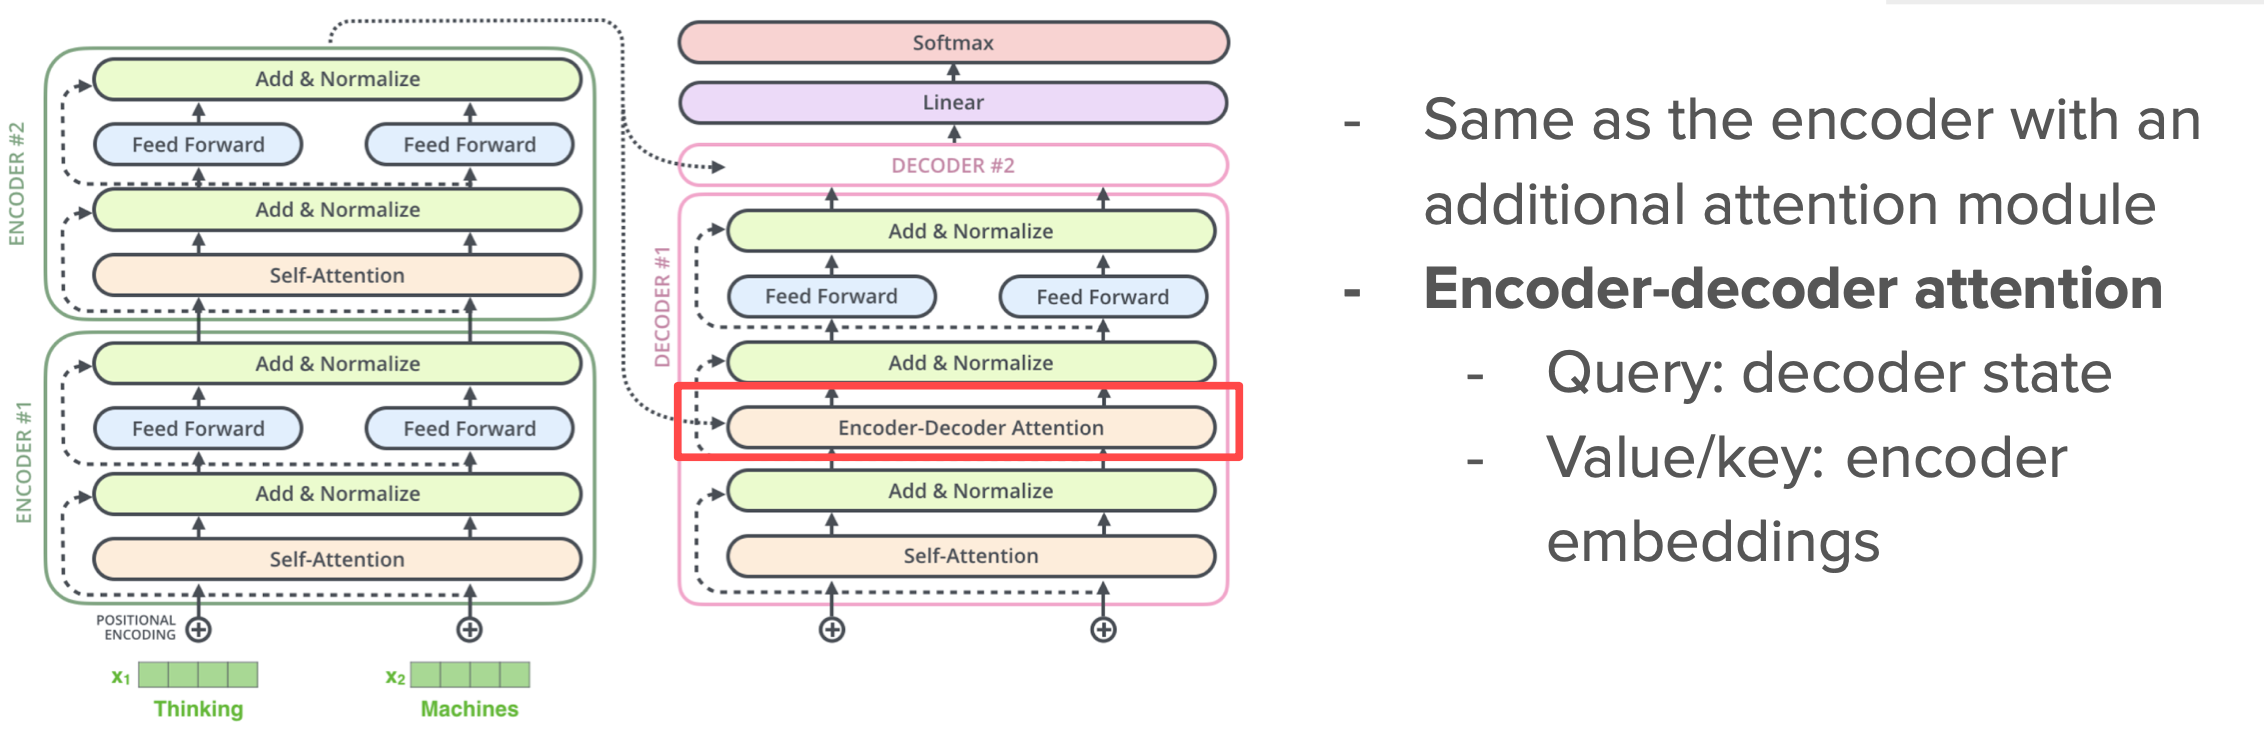
\includegraphics[width=\textwidth]{figures/decoder}
    \end{figure}
    \begin{itemize}
                        \item Autoregressive generation
                        \item Self-attention over prefix, encoder-decoder attention over inputs
                \item Output at each position:
                    $$
                    p(y_t\mid x, y_{1:t-1})
                    $$
                \item MLE training
    \end{itemize}
\end{frame}

%\begin{frame}
%    {Transformer as an encoder-decoder model}
%    \begin{columns}
%        \begin{column}{.4\textwidth}
%    \begin{figure}
%        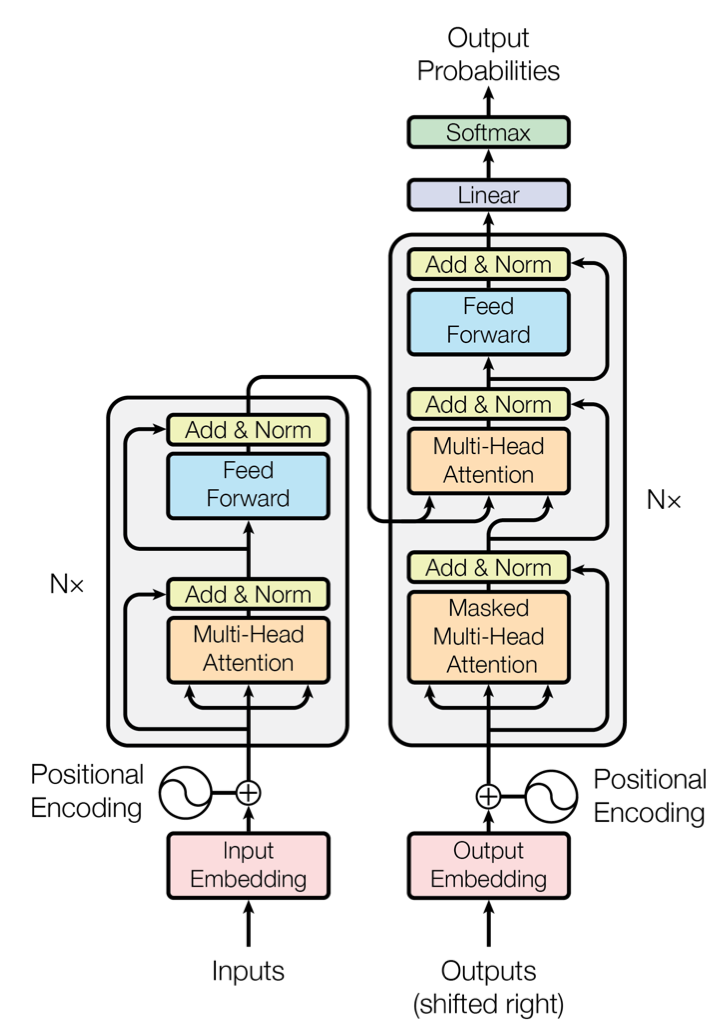
\includegraphics[height=7cm]{figures/transformer}
%    \end{figure}
%        \end{column}
%        \begin{column}{.6\textwidth}
%            \begin{itemize}
%                \item Stacked transformer block
%                \item Decoder attention:
%                    \begin{itemize}
%                        \item Autoregressive generation
%                        \item Self-attention over prefix
%                        \item Encoder-decoder attention over inputs
%                    \end{itemize}
%                \item Output at each position:
%                    $$
%                    p(y_t\mid x, y_{1:t-1})
%                    $$
%                \item MLE training
%            \end{itemize}
%        \end{column}
%    \end{columns}
%\end{frame}

\begin{frame}
    {Impact on NLP}
    \begin{itemize}
        \item Initially designed for sequential data and obtained SOTA results on MT
        \item Replaced recurrent models (e.g. LSTM) on many tasks
        \item Enabled large-scale training which led to pre-trained models such as BERT and GPT-2
    \end{itemize}

    Limitation: fixed length input (see Longformer, Performer etc.)
\end{frame}

\section{Pre-trained models}

\begin{frame}
    {Representation learning}
    What are good representations?\\
    \begin{itemize}
        \item[] Contains good features for downstream tasks 
    \end{itemize}
    Example:
    \vspace{-1em}
    \begin{table}
        \begin{tabular}{ll}
            negative & the food is good but doesn't worth an hour wait
        \end{tabular}
    \end{table}
    Simple features (e.g. BoW) require complex models.\\
    Good features only need simple (e.g. linear) models.
    \begin{figure}
        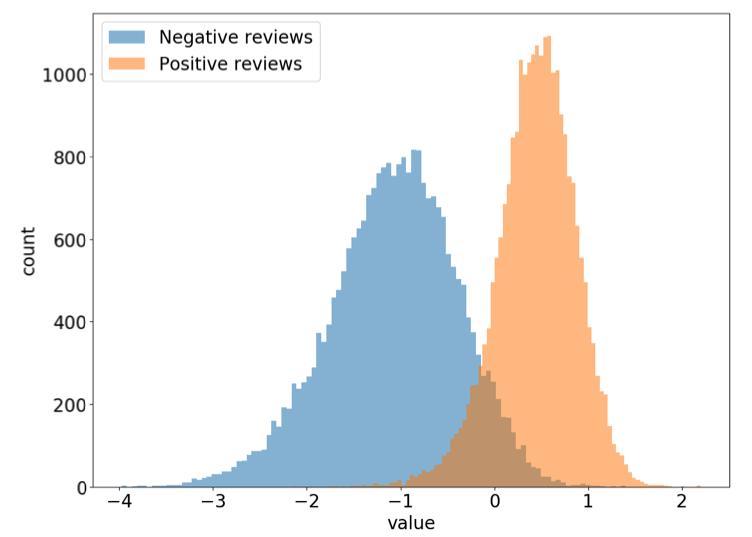
\includegraphics[height=3cm]{figures/sentiment}
        \caption{Sentiment neuron [Radford+ 2017]}
    \end{figure}
\end{frame}

\begin{frame}
    {Representation learning}
    Applications of good representations:\\
    \begin{itemize}
        \item Learning with small data: fine-tuning on learned representations
        \item Multi-task and transfer learning: one representation used for many tasks 
        \item Metric learning: get a similarity metric for free 
    \end{itemize}

    How do we learn the representations?
    \begin{itemize}
        \item Self-supervised learning: obtain representations through generative modeling
        %\item Auto-encoders: directy learn the mapping from input to a (latent) representation
    \end{itemize}
\end{frame}

\begin{frame}
    {Self-supervised learning}
    \beamerblue{Key idea}: predict parts of the input from the other parts
    \vspace{-2em}
    \begin{figure}
        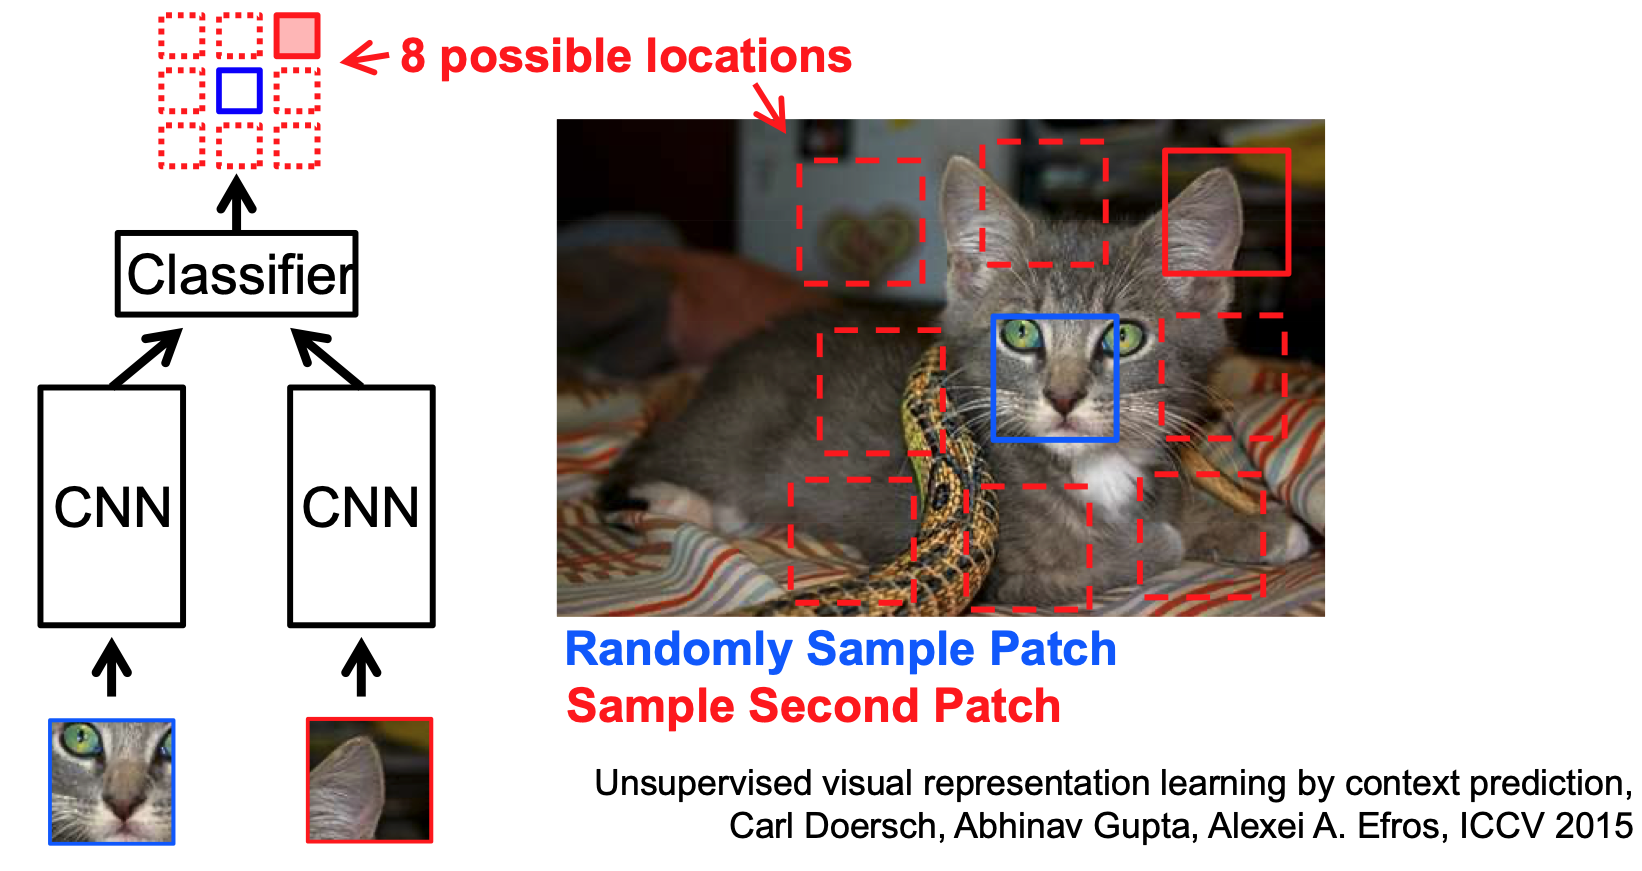
\includegraphics[height=5cm]{figures/image-self}
        \caption{Slide from Andrew Zisserman}
    \end{figure}
    \vspace{-2em}
    \begin{itemize}
        \item Other supervision signals: color, rotation etc.
        \item Video: predict future frames from past frames
    \end{itemize}
\end{frame}

\begin{frame}
    {Representation learning in NLP}
    Word embeddings\\
    \begin{itemize}
        \item CBOW, Skip-gram, GloVe, fastText etc.
        \item Used as the input layer and aggregated to form sequence representations
    \end{itemize}

    Sentence embeddings\\
    \begin{itemize}
        \item Skip-thought, InferSent, universal sentence encoder etc.
        \item Challenge: sentence-level supervision
    \end{itemize}

    Can we learn something in between?\\
    \begin{itemize}
        \item[] Word embedding with contextual information
    \end{itemize}
\end{frame}

\begin{frame}
    {Transfering knowledge from neural LM}
    Key idea: use representation from a generative model (i.e. an LM) \\
    \begin{itemize}
        \item Representation (e.g. hidden state at each word) is context-sensitive
        \item Contains relevant contextual information for predicting the next word
    \end{itemize}

    Early work:\\
    \begin{itemize}
        \item Fine-tune a recurrent LM for downstream tasks [Dai+ 2015, Howard+ 2018]
        \item Use word embedding from a pre-trained LM in addition to standard word embedding [Peters+ 2017]
        \item Promising results on a smaller scale
    \end{itemize}

    Embeddings from language models (ELMo) [Peters+ 2018]\\
    \begin{itemize}
        \item Use word embeddings from a bi-directional LM
        \item Success on multiple NLP tasks
    \end{itemize}
\end{frame}

\begin{frame}
    {ELMo pretraining}
        Forward/backward language models:\\
            \begin{itemize}
                \item $p_{\text{fwd}}(x) = \prod_{t=1}^T p(x_t\mid \underbrace{x_{1:t-1}}_{\text{past}}; \theta_{\text{fwd}})$
                \item $p_{\text{bwd}}(x) = \prod_{t=T}^1 p(x_t\mid \underbrace{x_{t+1:T}}_{\text{future}}; \theta_{\text{bwd}})$
                \item Each LM is a two layer LSTM,
                with shared input embedding layer and softmax layer
            \end{itemize}

        Subword representation:\\
            \begin{itemize}
                \item First layer word embedding is from character convolutions
            \end{itemize}

        Data: one-billion word benchmark (monolingual data from WMT)
\end{frame}

\begin{frame}
    {ELMo embeddings}
    Contextual embeddings capture word senses.
    \begin{figure}
        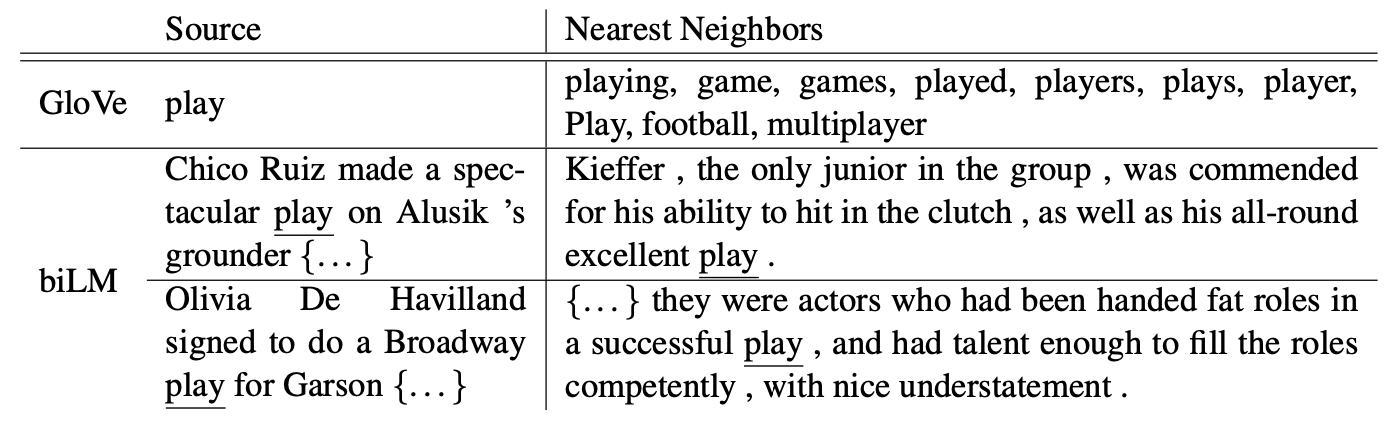
\includegraphics[width=.9\textwidth]{figures/elmo-ex}
        \caption{From [Peters+ 2018].}
    \end{figure}
\end{frame}

\begin{frame}
    {ELMo Fine-tuning}
    Obtain contextual word embeddings from each layer $j\in{0, \ldots, L}$ of biLM:
    $$
        \text{Embed}(x_t, j) = \begin{cases}
            [\overrightarrow{h}_{t,j}; \overleftarrow{h}_{t,j}] & \text{ for } j > 0 \\
            \text{CharEmbed}(x_t) & \text{ for } j = 0
        \end{cases}
    $$
    Task-specific combination of embeddings:
    $$
    \text{Embed}(x_t) = \gamma \sum_{j=0}^L w_j\text{Embed}(x_t, j)
    $$

    Fix biLM and use the contextual word embeddings as input to task-specific models. (Can also add to the output layer.)

    Regularization is important: $L_2$ or dropout.
\end{frame}

\begin{frame}
    {ELMo results}
    Improvement on a wide range on NLP tasks:\\
    \begin{itemize}
        \item \emph{reading comprehension} (SQuAD)
        \item entailment/natural language inference (SNLI)
        \item semantic role labeling (SRL)
        \item coreference resolution (Coref) 
        \item \emph{named entity recognition} (NER) 
        \item sentiment analysis (SST-5)
    \end{itemize}
    \vspace{-2em}
    \begin{figure}
        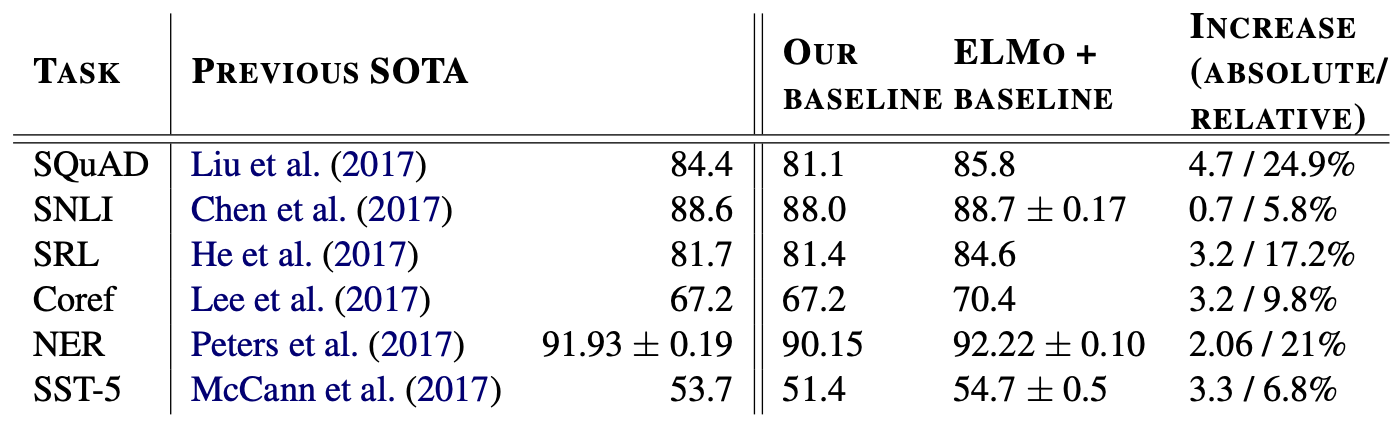
\includegraphics[width=.9\textwidth]{figures/elmo-res}
    \end{figure}
\end{frame}

\begin{frame}
    {Takeaways}
    \begin{itemize}
        \item Main idea: use biLM for representaiton learning
        \item Outputs from all layers are useful
            \begin{itemize}
                \item Lower layer is better for syntactic tasks, e.g. POS tagging, parsing
                \item Hight layer is better for semantic tasks, e.g. question answering, NLI
                \item Some fine-tuning of the pre-trained model is needed.
            \end{itemize}
        \item \emph{Large-scale training} is important
    \end{itemize}
    Next, pre-trained transformer models.
\end{frame}

\begin{frame}
    {Transformer models}
    \begin{figure}
        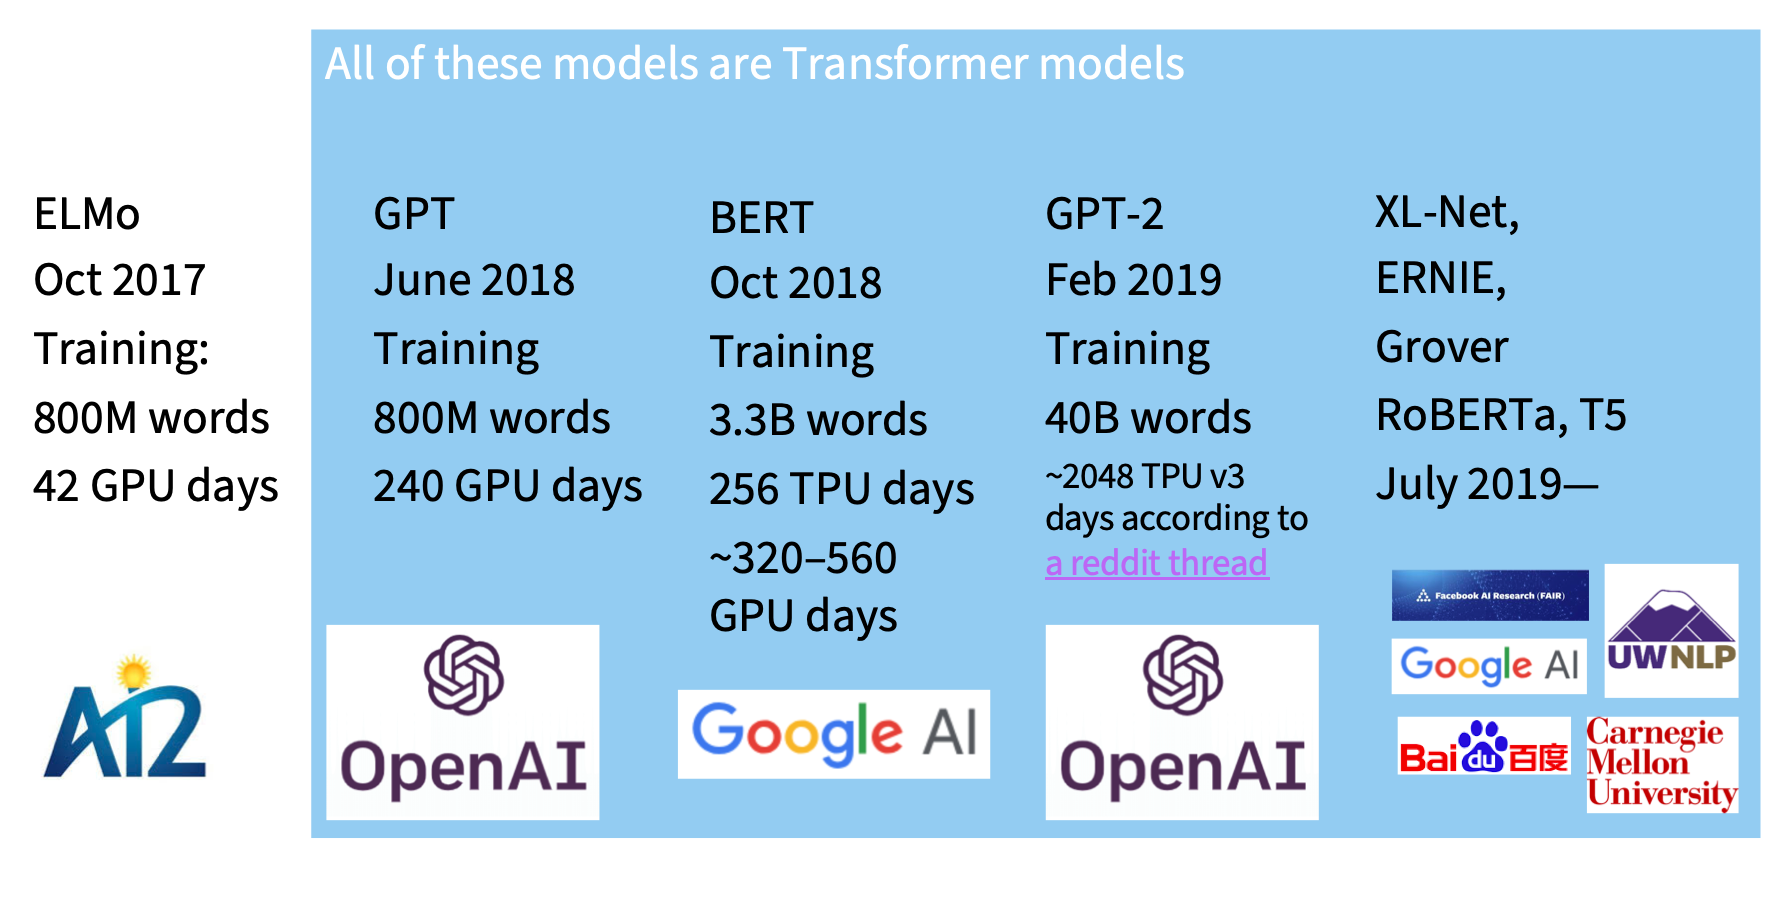
\includegraphics[width=0.9\textwidth]{figures/transformers}
        \caption{Slide from Chris Manning}
    \end{figure}
\end{frame}

\begin{frame}
    {Bidirectional Encoder Representations from Transformers (BERT)}
    Pre-training:\\
    \begin{enumerate}
        \item Masked LM: $$\BE_{x\sim\sD, i\sim p_{\text{mask}}} \log p(x_i\mid x_{-i}; \theta)$$ (not a LM)
            \begin{itemize}
                \item $x_{-i}$: noised version of $x$ where $x_i$ is replaced by \texttt{[MASK]}, a random token, or the original token
                \item $p(x_i\mid x_{-i}; \theta) = \text{Transformer}(x_{-i}, i)$
            \end{itemize}
        \item Next sentence prediction:
            $$
            \BE_{x^1 \sim\sD, x^2\sim p_{\text{next}}} \log p(y\mid x^1, x^2)
            $$
            \begin{itemize}
                \item $y$: whether $x^2$ follows $x^1$
                \item Not as useful as masked LM
            \end{itemize}
    \end{enumerate}
\end{frame}

\begin{frame}
    {BERT sentence pair encoding}
    \begin{figure}
            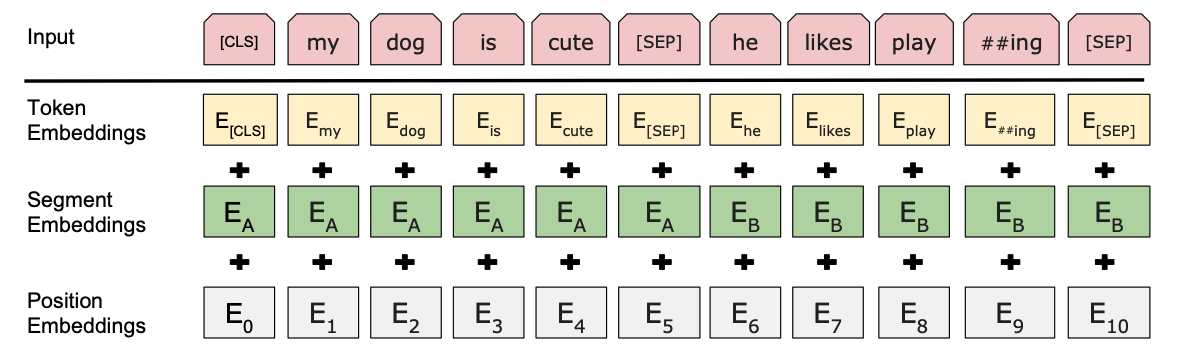
\includegraphics[width=.9\textwidth]{figures/bert}
    \end{figure}
    \begin{itemize}
        \item \texttt{[CLS]}: first token of all sequences; used for next sentence prediction
        \item Distinguish two sentences in a pair: \texttt{[SEP]} and segment embedding
        \item Learned position embedding
        \item Subword unit: wordpiece (basically byte pair encoding) 
    \end{itemize}
\end{frame}

\begin{frame}
    {BERT fine-tuning}
    All weights are fine-tuned (with a small learning rate)
    \vspace{-1.5em}
    \begin{figure}
            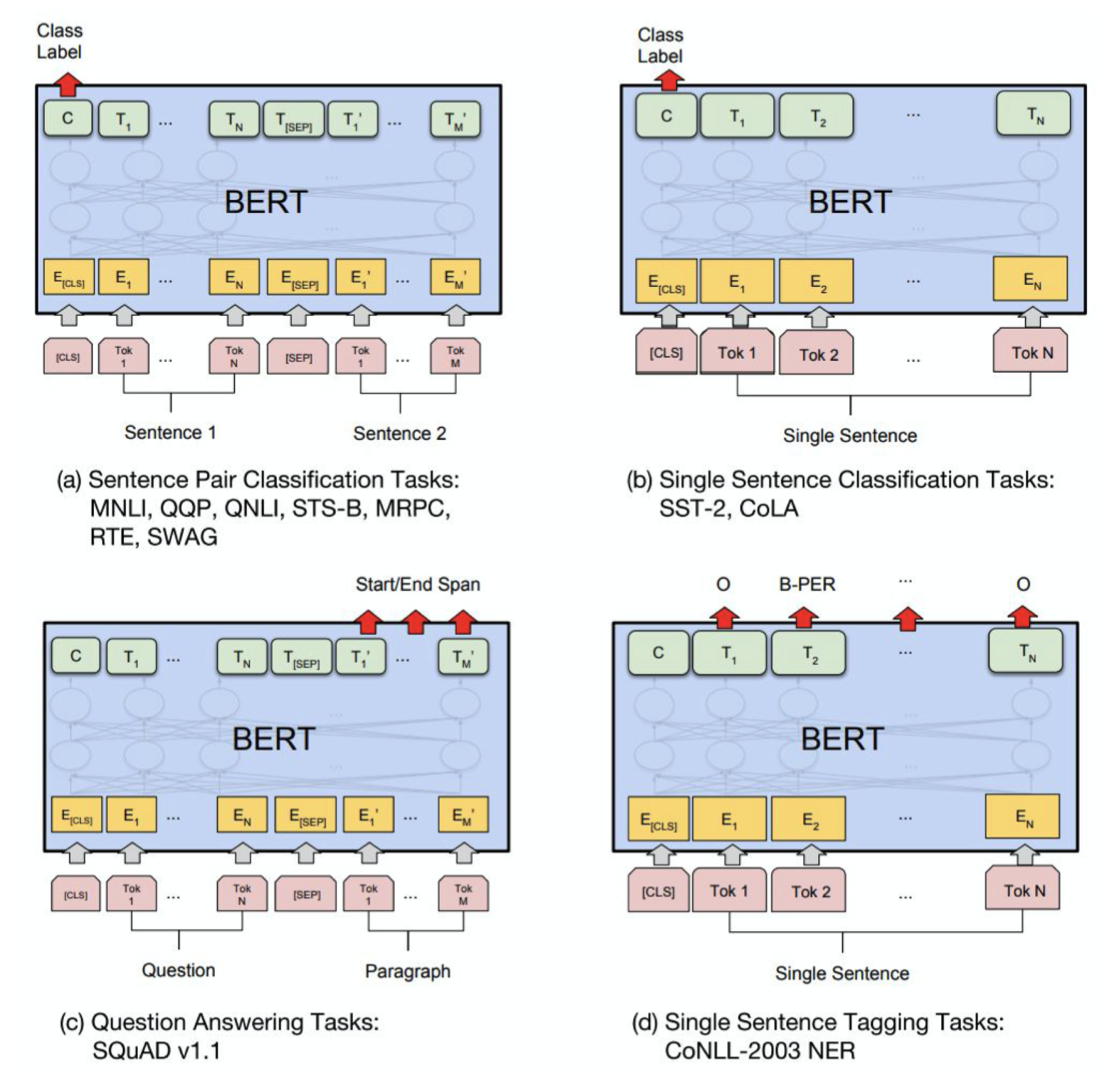
\includegraphics[height=0.9\textheight]{figures/bert-finetuning}
    \end{figure}
\end{frame}

\begin{frame}
    {Recent progress}
    GLUE: benchmark of natural language understanding tasks
    \begin{figure}
            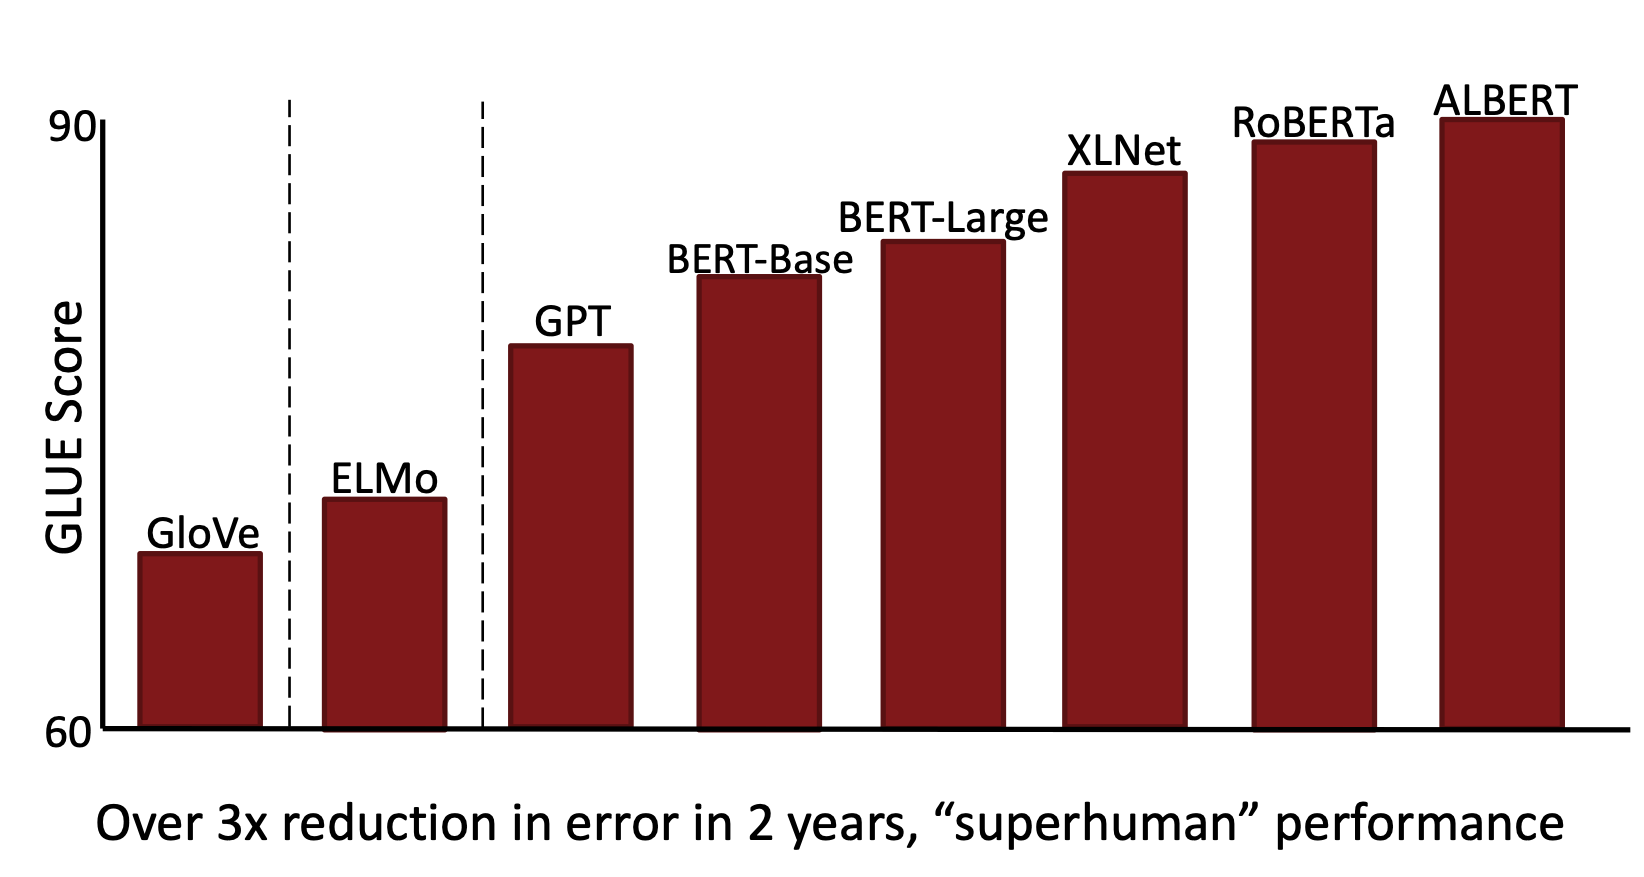
\includegraphics[width=.8\textwidth]{figures/glue}
            \caption{Slide from Chris Manning}
    \end{figure}
\end{frame}

\begin{frame}
    {The new pre-train then fine-tune paradigm}
    \begin{figure}
            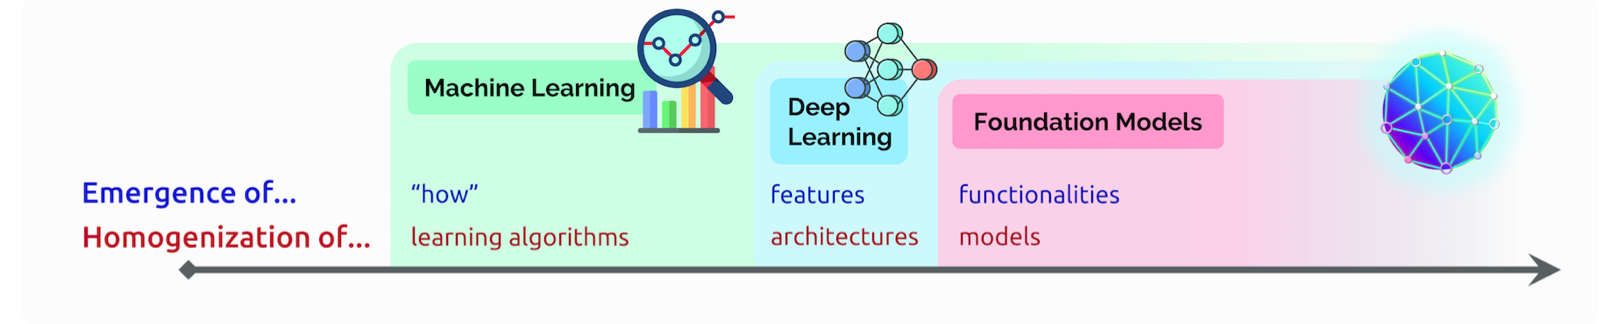
\includegraphics[width=.9\textwidth]{figures/homogenization}
            \caption{[Bommasani et al., 2021]}
    \end{figure}
    \begin{itemize}
\item \emph{One model} to absorb large amounts of raw data from various domains and modalities
\item Then \emph{adapted} to different downstream tasks
    \end{itemize}
\end{frame}

\begin{frame}
    {Summary}
    Off-the-shelf solution for NLP tasks: fine-tune BERT (and friends)

    What's next?\\
    \begin{itemize}
        \item Processing long text
        \item Efficient training/inference
        \item Learning with a small amount of data
        \item Robustness to distribution shifts
    \end{itemize}
\end{frame}

\section{Scaling up pre-trained models}
\begin{frame}
    {In-context learning}
    GPT-3 by OpenAI: Transformer-based LM with 175B parameters

    Zero-shot learning given task instruction / prompt:
    \begin{figure}
            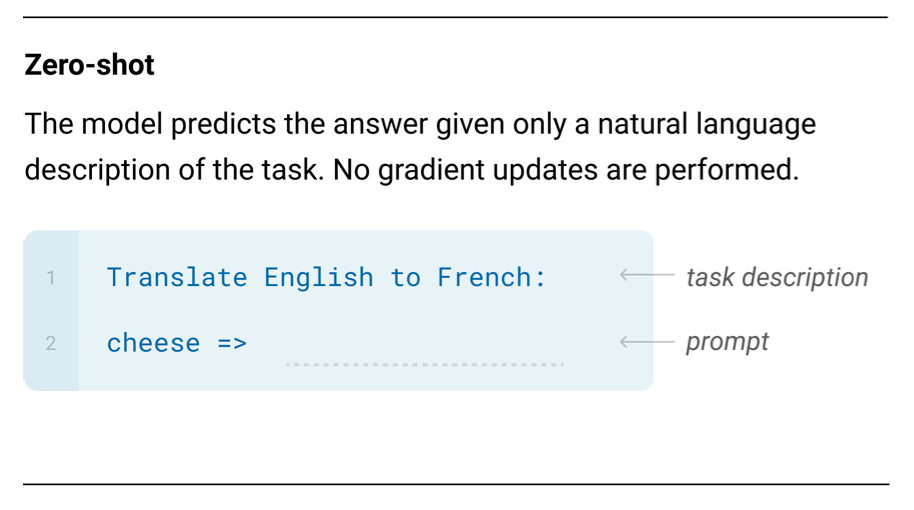
\includegraphics[height=6cm]{figures/in-context-zero}
    \end{figure}
\end{frame}

\begin{frame}
    {In-context learning}
    Few-shot learning with in-context examples (with no gradient update):
    \begin{figure}
            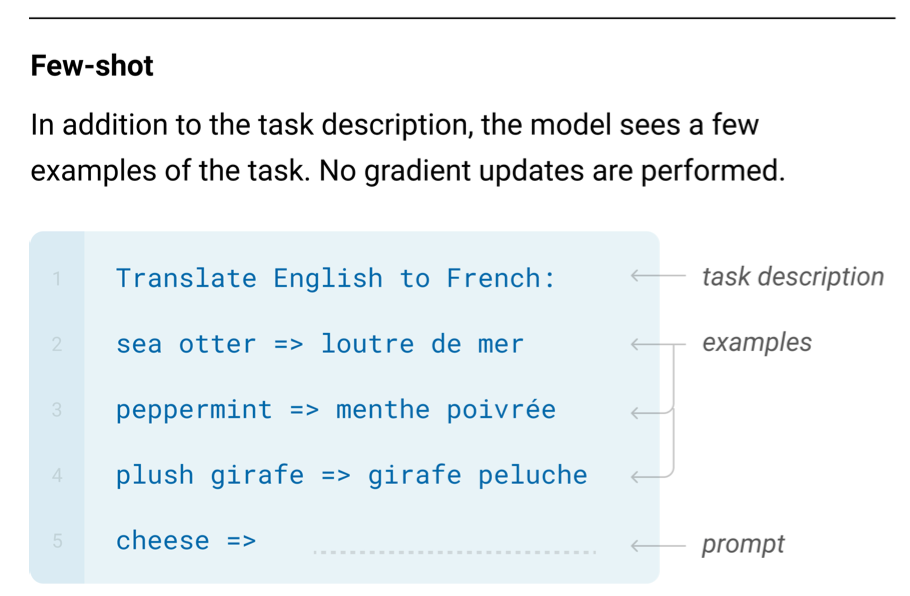
\includegraphics[height=6cm]{figures/in-context-few}
    \end{figure}
\end{frame}

\begin{frame}
    {In-context learning}
    Larger models make increasingly efficient use of in-context information
    \begin{figure}
            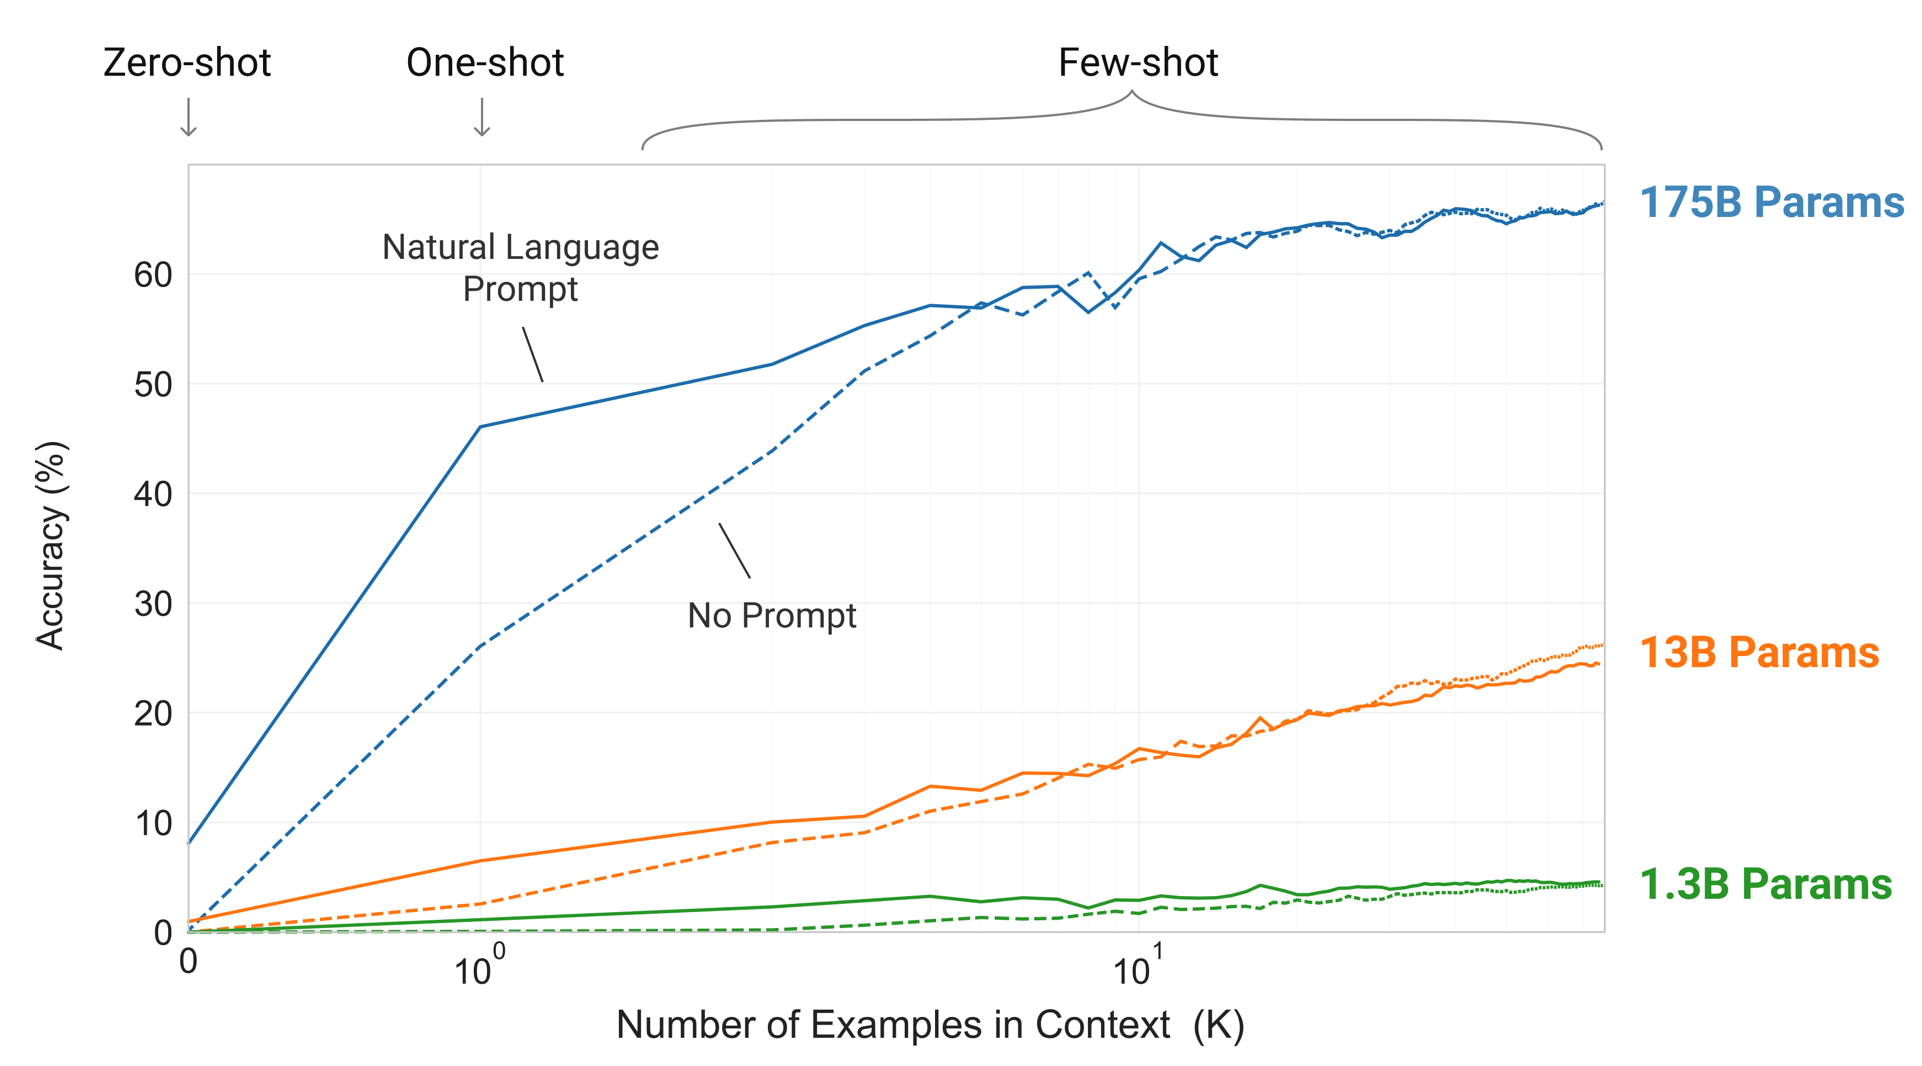
\includegraphics[height=6cm]{figures/scaling}
    \end{figure}
\end{frame}

\begin{frame}
    {In-context learning}
    Pre-trained LMs can be adapted for multimodal learning too:
    \begin{figure}
            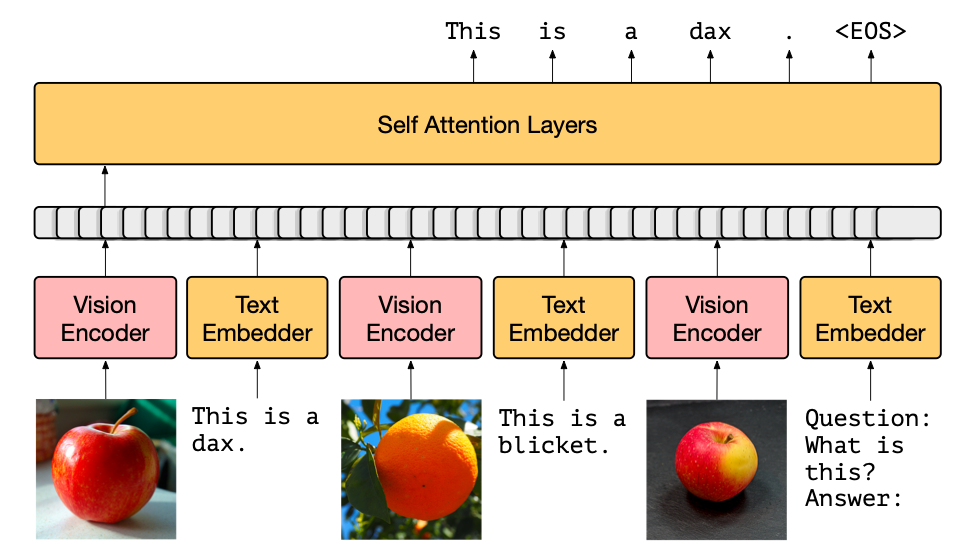
\includegraphics[height=5cm]{figures/in-context-multimodal}
            \caption{Multimodal Few-Shot Learning with Frozen Language Models}
    \end{figure}
    \vspace{-1em}
    Text embedder and self-attention use frozen weights from pre-trained LM.
\end{frame}

\begin{frame}
    {Language modeling is all you need?}
    Text-to-text framework:
    \begin{figure}
            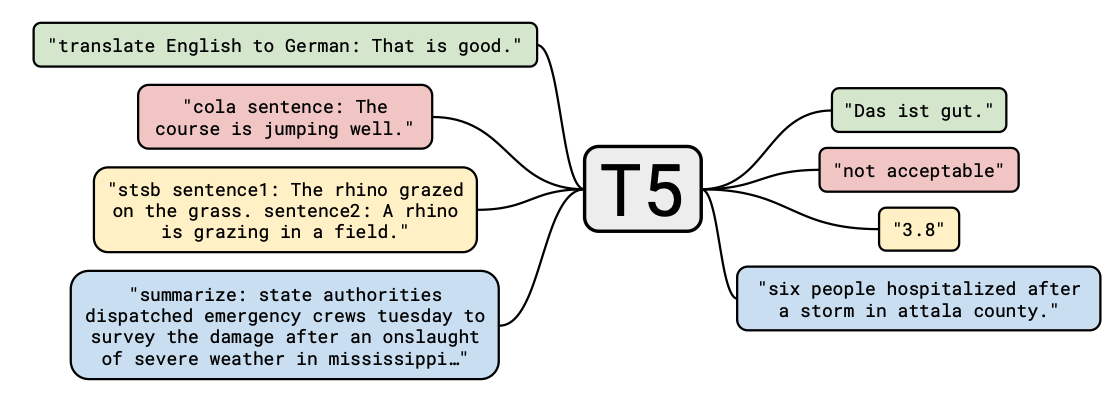
\includegraphics[height=5cm]{figures/t5}
            \caption{Exploring the Limits of Transfer Learning with a Unified Text-to-Text Transformer}
    \end{figure}
\end{frame}

\begin{frame}
    {Discussion: what can go wrong?}
\end{frame}

%\section{Autoencoders and VAEs}
%
%\begin{frame}
%    {Overview}
%    \beamerblue{Motivation}: Directly learn a (parametric) mapping from the input to the representation
%
%    \beamerblue{Encoder}: dimensionality reduction (data to code)
%    $$z = \text{enc}_\theta(x)$$
%
%    \beamerblue{Decoder}: reconstruction (code to data)
%    $$x = \text{dec}_\gamma(\text{enc}_\theta(x)) $$
%
%    \beamerblue{Learning}: reconstruction loss
%    $$
%    J(\theta, \gamma) = \frac{1}{|\sD|}\sum_{x\in\sD} L(x, \text{dec}_\gamma(\text{enc}_\theta(x)))
%    $$
%    \vspace{-1em}
%    $L$: MSE, cross-entropy etc.
%\end{frame}
%
%\begin{frame}
%    {Autoencoder}
%    \vspace{6em}
%    \begin{itemize}
%        \item Parametrize encoder and decoder by neural networks
%        \item What model can we use if $x$ is text?
%        \item \alert{Problem}: $z$ could just copy the input $x$ and no meaningful representation is learned!
%    \end{itemize}
%\end{frame}
%
%\begin{frame}
%    {Denoise autoencoder}
%    \beamerblue{Intuition}: structural information is needed to recover a corrupted input
%
%    \beamerblue{Learning}: reconstruction clean input from a corrputed version
%    $$
%    J(\theta, \gamma) = \frac{1}{|\sD|}\sum_{x\in\sD} \BE_{\tilde{x}\sim p_c(\cdot\mid x)}\pb{L(x, \text{dec}_\gamma(\text{enc}_\theta(\tilde{x})))}
%    $$
%
%    \begin{itemize}
%        \item Corruption: delete/insert/substitute words, Gaussian noise for images
%        \item Which model we have seen can be considered as a denoise autoencoder? 
%    \end{itemize}
%\end{frame}
%
%\begin{frame}
%    {Variational autoencoder}
%    Model $z$ as a latent variable: $$p(x;\theta) = \sum_{z\in\sZ} p(x, z;\theta)
%    \quad (\int_z p(x,z;\theta)dz \quad \text{if $z$ is continuous})
%    $$
%
%    Recall the evidence lowerbound (see lecture on EM)
%    \begin{align*}
%        \text{ELBO} &= \log p(x; \theta) - \KL{q(z)}{p(z\mid x;\theta)} \\
%        &= \sum_{z\in\sZ} q(z)\log \frac{p(x,z;\theta)}{q(z)}
%    \end{align*}
%
%    Concept check: What is $q(z)$ for EM?
%
%    In general, we can learn $q(z)$ for each sample:
%    $$
%    \max_\theta \sum_{x\in\sD} \max_\gamma \sum_{z\in\sZ} q(z;\gamma)\log \frac{p(x,z;\theta)}{q(z;\gamma)}
%    $$
%\end{frame}
%
%\begin{frame}
%    {Variational autoencoder}
%    Objective:
%    $$
%    \max_\theta \sum_{x\in\sD} \max_\gamma \sum_{z\in\sZ} q(z;\gamma)\log \frac{p(x,z;\theta)}{q(z;\gamma)}
%    $$
%    EM-style learning:\\
%    \begin{enumerate}
%        \item Solve $\gamma$ for each sample (using SGD):
%            $$\gamma^*_x \leftarrow \max_\gamma \text{ELBO}(x;\theta^{\text{old}}, \gamma)$$ 
%        \item One-step update $\theta^{\text{old}}$:
%            $$\theta^{\text{new}} \leftarrow \theta^{\text{old}} + \nabla_\theta\sum_{x\in\sD}\text{ELBO}(x;\theta, \gamma^*_x)$$
%    \end{enumerate}
%    Problems:\\
%    \begin{itemize}
%        \item Step 1 is expensive!
%        \item How to compute the gradient?
%    \end{itemize}
%\end{frame}
%
%\begin{frame}
%    {Amortized variational inference}
%    \beamerblue{Problem}: finding the optimal variation distribution for each sample $x$ is expensive
%            $$\gamma^*_x \leftarrow \max_\gamma \text{ELBO}(x;\theta^{\text{old}}, \gamma)$$ 
%
%    \beamerblue{Idea}: learn the mapping $f_\phi\colon x \rightarrow \gamma^*_x$ 
%
%    Note that $f_\phi(x)$ specifies the distribution $q(z;\gamma_x)$.
%    Let's use $q(z\mid x;\phi)$ to denote $q_\gamma(z)$.
%
%    Estimate $\phi$ (same for all $x$)
%    \begin{align*}
%        & \max_\phi \sum_{x\in\sD}\text{ELBO}(x;\theta, \phi)\\
%        &= \max_\phi \sum_{x\in\sD} \BE_{q(z\mid x; \phi)} \pb{\log \frac{p(x,z;\theta)}{q(z\mid x;\phi)}}
%    \end{align*}
%    Update $\phi$ and $\theta$ iteratively for each mini-batch.
%\end{frame}
%
%\begin{frame}
%    {Gradient computation}
%    Need to compute $\nabla_\phi \text{ELBO}(x;\phi,\theta)$ and $\nabla_\theta \text{ELBO}(x;\phi,\theta)$
%
%    Monte Carlo sampling (REINFORCE):
%    \begin{align*}
%    \nabla_\phi \BE_{q(z\mid x; \phi)} \pb{\log \frac{p(x,z;\theta)}{q(z\mid x;\phi)}}
%        &= \BE_{q(z\mid x; \phi)} \pb{\nabla_\phi q(z\mid x; \phi)  \log \frac{p(x,z;\theta)}{q(z\mid x;\phi)}} \\
%        &\approx \frac{1}{n}\sum_{i=1}^n \pb{\nabla_\phi q(z^{(i)}\mid x; \phi)  \log \frac{p(x,z^{(i)};\theta)}{q(z^{(i)}\mid x;\phi)}}
%    \end{align*}
%    where $z^{(i)}\sim q(z\mid x; \phi)$.
%
%    Problem: gradient estimator has \alert{high variance}.
%\end{frame}
%
%\begin{frame}
%    {Reparametrization trick}
%    \begin{figure} 
%        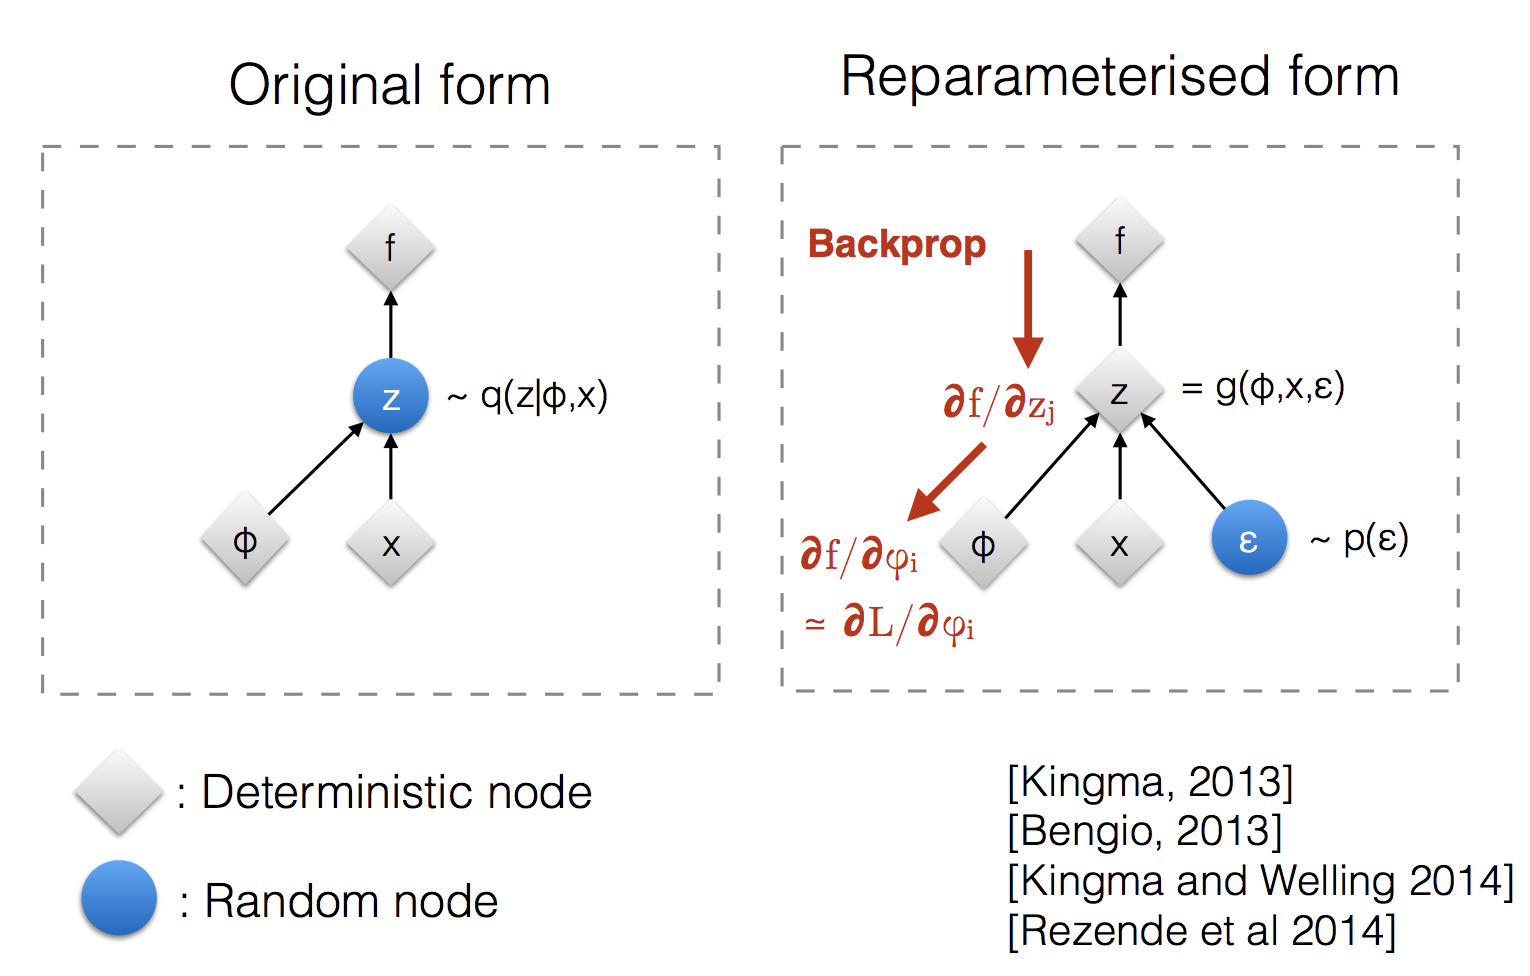
\includegraphics[width=.7\textwidth]{figures/reparam}
%    \end{figure}
%    \vspace{-1em}
%    Original distribution: $z^{(i)}\sim q(z\mid x; \phi)$\\
%    Auxiliary independent random variable: $\epsilon\sim p(\epsilon)$ \\
%    Reparametrization trick: $z = \sT(\epsilon, x; \phi)$
%\end{frame}
%
%\begin{frame}
%    {Parametrization by neural networks}
%    \begin{figure}
%        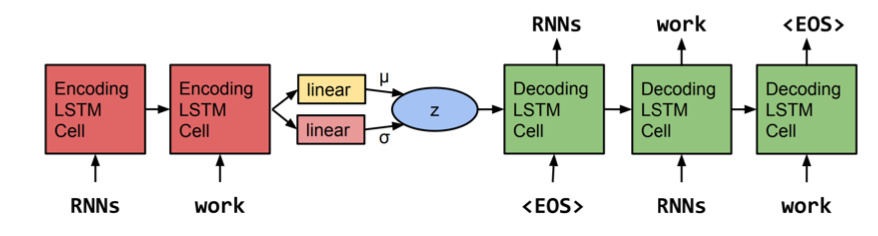
\includegraphics[width=.8\textwidth]{figures/vae}
%    \end{figure}
%    \vspace{-1em}
%    Joint distribution: $p(x,z;\theta) = p(x\mid z;\theta) p(z;\theta)$
%
%    Prior: $p(z;\theta) = \sN(z\mid 0, I)$
%
%    Likelihood: $p(x\mid z;\theta) = \text{dec}_\theta(z)$
%
%    Variational distribution: $q(z\mid x; \phi) = \text{enc}_\phi(x) = \mu_\phi(x), \sigma^2_\phi(x)$
%
%    Reparametrization:
%    \begin{align*}
%        \epsilon &\sim \sN(0, I) \\
%        z &= \mu_\phi(x) + \sigma^2_\phi(x)\cdot \epsilon
%    \end{align*}
%\end{frame}
%
%\begin{frame}
%    {Summary}
%    \begin{itemize}
%        \item Autoencoders: directly learn a low-dimensional representation through reconstruction
%        \item VAEs: impose structure on the latent representation
%            \begin{itemize}
%                \item In addition to representation learning, also used for latent variable models in NLP
%                \item Issues: posterior collapse, evaluation 
%            \end{itemize}
%    \end{itemize}
%\end{frame}

\end{document}
